\documentclass[11pt]{ucthesis}
\setlength{\oddsidemargin}{0.15in}
\def\dsp{\def\baselinestretch{1.75}\large\normalsize}
\ssp
\usepackage{amsmath}
\usepackage[pdftex]{graphicx}
\usepackage{times}
%\usepackage[cmex10]{amsmath}
\usepackage{amsfonts}
\usepackage[usenames,dvipsnames]{color}
%\usepackage{array}
%\usepackage{mdwmath}
%\usepackage{mdwtab}

\usepackage{verbatim}
\usepackage{fancyvrb, relsize}
\usepackage{url}
\usepackage{hyperref}

\newcommand{\rt}{real-time}
\newcommand{\Rt}{Real-time}
\newcommand{\thdint}{thread-interleaved}
\newcommand{\Thdint}{Thread-interleaved}

\newcommand{\todo}[1]{{{\textcolor{Red}{(Todo: #1)}}}}%

\begin{document}
\title{Precision Timed Machines
\iffalse
From Ptides to PtidyOS, Designing Distributed Real-Time Embedded Systems
  \titlenote{This work was supported in part by the Center for Hybrid and Embedded Software Systems (CHESS) at UC Berkeley, which receives support from the National Science Foundation (NSF awards \#0720882 (CSR-EHS: PRET), \#0931843 (ActionWebs), and \#1035672 (CSR-)CPS Ptides)), the U. S. Army Research Office (ARO \#W911NF-07-2-0019), the U. S. Air Force Office of Scientific Research (MURI \#FA9550-06-0312), the Air Force Research Lab (AFRL), the Multiscale Systems Center (MuSyC), one of six research centers funded under the Focus Center Research Program, a Semiconductor Research Corporation program, and the following companies: Bosch, National Instruments, Thales, and Toyota.}
\fi
}
\author{Isaac Liu} 
\degreeyear{2012}
\degreesemester{Spring}
\degree{Doctor of Philosophy}
\chair{Professor Edward A. Lee}
\othermembers{Professor John Wawrzynek \\
Professor Alice Agogino}
\numberofmembers{3}
\prevdegrees{Bachelor of Science (University of California, Santa Barbara) 2007}
\field{Electrical Engineering and Computer Science}
\campus{Berkeley}

\maketitle
%FIXME for the final version, comment out the approval page.
%\approvalpage
\copyrightpage

\begin{abstract}
Cyber-Physical Systems (CPS) are integrations of computation with physical processes~\cite{Lee08_CyberPhysicalSystemsDesignChallenges}.
%A number of applications can benefit from the potential of CPS. 
These systems must be equipped to handle the inherent concurrency and inexorable passage of time of physical processes.  
Traditional computing abstractions only concern themselves with the �functional� aspects of a program, and not its timing properties.
Thus, nearly every abstraction layer has failed to incorporate \emph{time} into its semantics; the passage of time is merely a consequence of the implementation. 
When the temporal properties of the system must be guaranteed, designers must reach beneath the abstraction layers.
This not only increases the design complexity and effort, but the systems are overdesigned, brittle and extremely sensitive to change.

In this work, we address the difficulties of handling \emph{time} in computing systems by re-examining the lower levels of abstraction. 
In particular, we focus on the instruction set architecture (ISA) layer and its affects on microarchitecture design.
The ISA defines the contract between software instructions and hardware implementations. 
Modern ISAs do not constrain timing properties of instructions as part of the contract. 
Thus, architecture designs have largely implemented techniques that improve average performance at the expense of execution time variability.
This leads to imprecise WCET bounds that limit the timing predictability and timing composability of architectures.  

In order to address the lack of temporal semantics in the ISA, we propose instruction extensions to the ISA that give temporal meaning to the program. 
The instruction extensions allow programs to specify execution time properties in software that must be observed for any \emph{correct} execution of the program.
These include the ability to specify a minimum execution time for code blocks, and the ability to detect and handle missed deadlines from code blocks that exhibit variable execution times.
This brings control over timing to the software and allows programs to contain timing properties that are independent of the underlying architecture.   
In addition, we present the Precision Timed ARM (PTARM) architecture, a realization of Precision Timed (PRET) machines~\cite{edwards2007case} that provides timing predictability and composability without sacrificing performance. 
PTARM employs a predictable thread-interleaved pipeline with an exposed memory hierarchy that uses scratchpads and a predictable DRAM controller. 
This removes timing interference among the hardware threads, enabling timing composability in the architecture, and provides deterministic execution times for instructions within the architecture, enabling timing predictability in the architecture.  
We show that the predictable thread-interleaved pipeline and DRAM controller design also achieve better throughput compared to conventional architectures when fully utilized, accomplishing our goal to provide both predictability and performance.  

To show the applicability of the architecture, we present two applications implemented with the PRET architecture that utilize the predictable execution time and the extended ISA to achieve their design requirements. 
The first application is a real-time fuel rail simulator that implements a one dimensional computational fluid dynamics (1D-CFD) solver on a multicore PRET architecture.
The implementation leverages the timing instructions to synchronize the communication of multiple PRET cores with low overhead. 
The predictable nature and the improved throughput of the architecture allow us to optimize the resource usage while statically ensuring that the timing requirements are met.
This provides a scalable solution to close the loop of fuel delivery, allowing for more precise fuel injections that lead to a cleaner and more efficient engine.
The second application presents a case study that uses PRET to remove the vulnerability of timing side-channel attacks on encryption algorithms.
Encryption algorithms are vulnerable to side-channel attacks that measure the execution time of the encryption to derive the encryption key. 
The uncontrollable execution time variance can stem from the unpredictable sharing of architecture features or from the various control paths of the encryption algorithm. 
We implement the RSA and DSA~\cite{dss} encryption algorithms on PRET and show that by using the timing extended ISA and a predictable architecture, we can completely remove the vulnerabilities that are exploited for the attacks.

By providing a predictable architecture, we provide simpler and more accurate timing analysis of the software.  
With the instruction extensions to the ISA, we provide timing control and allow architecture independent timing properties to be specified in the software. 
Through these contributions, we aim to introduce a timing deterministic foundation to the lower levels of computing abstractions, which enables more precise and efficient control over timing for the design of CPS.



\end{abstract}

\begin{frontmatter}

\begin{dedication}
\null\vfil
{\large
\begin{center}
%\\\vspace{12pt}
To my wife Emily Cheung, my parents Char-Shine Liu and Shu-Jen Liu, and everyone else whom
I've had the pleasure of running into for the first twenty-seven years of my
life.
%\\\vspace{12pt}
\end{center}}
\vfil\null
\end{dedication}

\tableofcontents
\listoffigures
\listoftables
\begin{acknowledgements}

I want to thank my wife

I want to thank my parents

I want to thank my advisor, Edward A. Lee

I want to thank the committee members

I want to thank Hiren Patel

I want to thank Jan Rieneke

I would also like to thank the ptolemy group especially Christopher and Mary, Jia for providing me the template

I would like to thank everyone else that made this possible

\end{acknowledgements}

\end{frontmatter}

\chapter{Introduction}
\label{chapter:intro}
%Cyber physical systems - different than traditional embedded systems that interact with real world. Timing requirements, but large, and safety critical
\section{Motivation}
\emph{Cyber-Physical Systems} (CPS) are integrations of computation with physical processes~\cite{Lee08_CyberPhysicalSystemsDesignChallenges}.
In these systems, computation and physical process often form a tight feedback loop, affecting the behavior of each other.
The embedded platforms and networks employed not only control the physical process, but at the same time monitor and adapt to the changes of the physical process.
An enormous number of applications can be categorized as CPS.
They include high confidence medical devices and systems, assisted living, traffic control and safety, advanced automotive systems, process control, energy conservation, environmental control, avionics, instrumentation, critical infrastructure control (electric power, water resources, and communications systems for example), distributed robotics (telepresence, telemedicine), defense systems, manufacturing, and smart structures.
However, in order for CPS to be deployed in high confidence systems, such as advanced automotive or avionics systems, the platforms employed need to deal with two important properties of the physical process: they are inherently concurrent, and time progresses at its own pace.
 
%modern design techniques are hitting a scalability wall - RTOS, compilers, general purpose architectures all create problems
%all layers need work. Modern abstraction layers omit time.. designers need to reach down below, can't certify a system with its hardware
% We deal with the ISA and architecture design

Traditionally, real-time embedded systems have dealt with the notion of time.
These systems impose deadlines and timing constraints to their underlying tasks to deliver services in real time. 
The timing constraints of \emph{soft real-time systems} are typically used to guarantee quality of service, while the constraints of \emph{hard real-time systems} are used to guarantee safety critical tasks, so they must be met. 
The real-time embedded community has widely adopted techniques developed for general purpose applications, believing that they will provide the same advantages and benefits for embedded systems.
These include the programing language, the operating system, the tool-chains, and the computer architecture.
However, these techniques are designed for general purpose systems that do not require stringent interaction with the physical environment. 
Thus, they place emphasis on improving average performance over predictability.   
As a result, when computing systems absolutely must meet tight timing constraints, these computing advances often do more harm than good~\cite{LeeOnTime2005}.
%this is contrary to reality~\cite{halang:DSP:2004:4,thiele:04:predictable}.
The scale and complexity of traditional embedded systems allow designers to compensate with extra effort in design and analysis. 
However, these solutions begin to break down when transitioning to larger scale CPS.   

In the current state of embedded software, nearly every abstraction has abstracted away \emph{time}.
The Instruction Set Architecture (ISA), meant to hide the hardware implementation details from the software, does not include timing semantics for the instruction executions.  
Widely adopted programming languages, meant to hide the details of the ISA from the program logic, do not express timing properties; timing is merely an accident of the implementation.
Real-time operating systems (RTOS), meant to hide the details of the program from their concurrent orchestration, often use priorities to dictate the execution of tasks; the execution time of tasks can easily affect the scheduled outcome of execution.
The lack of \emph{time} in the abstraction layers can lead to the following consequences:
\begin{itemize}
\item \emph{Unnecessary complexities in the interaction of concurrent components} --  
This often is manifested when components share resources. 
For example, software threads are the typical abstractions for concurrent software written in C or Java. 
Because there is no guarantee of when a shared variable will be accessed by each thread, locks and semaphores are required to avoid race conditions. 
This not only introduces bugs, but also introduces complex and almost impossible to analyze interactions between threads~\cite{leethreads}. 
As a result, there is great difficulty when synchronizing and communicating between components or tasks.

\item \emph{Unnecessary complexities in interactions across layers} -- 
For example, scheduling could be done at multiple levels simultaneously without any coordination. 
As tasks or software threads are scheduled for execution in the OS, an explicit multithreaded dynamic dispatch architecture could also be scheduling instructions from different hardware threads without the knowledge of the OS~\cite{thiele:04:predictable}.

\item \emph{Misleading or pessimistic analysis results when analyzing the whole system} -- 
For example, task scheduling and context switching cost may vary from the cache or pipeline state change after executing each tasks. 
This is often not factored into the analysis~\cite{thiele:04:predictable}. 
Furthermore, because the  large variation of execution time in modern complex processors, worst-case execution time (WCET) analysis techniques often lead to overly conservative results for safety~\cite{wilhelm-survey-paper}. 
As the WCET is often the basis for priority of any scheduling scheme, the conservativeness is propagated throughout the system.
\end{itemize}
%explain composability

When the temporal properties of the system must be guaranteed, designers must reach beneath the abstraction layers, and understand thoroughly the complex underlying details and its affect on execution time. 
This not only increases the design complexity and effort, but the designed systems are \emph{brittle} and extremely sensitive to change~\cite{Sangiovanni-Vincentelli2007automotive, edwards2007case}.  
For example, Sangiovanni-Vincentelli et al.\cite{Sangiovanni-Vincentelli2007automotive} show that when increasing the execution time of a task, any priority based scheduling scheme results in discontinuity in the timing of all tasks besides the task with the highest priority. 
At a lower level, adding a few instructions can easily result in a huge variation in program execution time; the state of the hardware dynamic prediction and speculation units, such as caches and pipelines, can easily be affected by small program additions.
Thus, in order to verify the timing of safety critical systems, the verification must be done on both the software system and its execution platform; they cannot be separated. 
This process is often time consuming and expensive.
Since the abstraction layers do not give any temporal semantics to the system, each layer must be completely understood in order to reason about and prove the timing properties of the full system.  
For avionics manufacturers, this means stockpiling the same hardware for the lifetime of an aircraft; any upgrade of components or software in their system could result in drastic timing changes, and thus require re-certification.


\subsection{Timing Predictable Systems}
Thiele et al.~\cite{thiele:04:predictable}, Henzinger~\cite{Henzinger2008} and Lee~\cite{LeeOnTime2005} have all identified the importance and difficulties of designing \emph{timing-predictable systems}.
Timing-predictable systems should exhibit the following property: \textit{a small change in the input must not result in a large change in the output}~\cite{Henzinger2008}.
If the definition of \emph{output} includes the timing behavior exhibited by the system, then current abstractions disrupts this property at almost all levels. 

A change is needed to efficiently and safely design next generation systems, especially if they effect the well being of our lives.
In particular, how software and hardware deal with the notion of \textit{time} needs to be more carefully understood and designed.
At the lowest levels of abstraction, circuits and microarchitectures, timing is central to correctness.
For example, in a microarchitecture, if the output of an ALU is latched at the wrong time, the ISA will not be correctly implemented.
However, at higher levels, for example, the ISA, timing is hidden, and there are no temporal semantics; the execution time is irrelevant to correctness. 
Thus, each abstraction layer needs to be revisited to judiciously introduce some form of temporal semantics. 
Specifically for CPS, platforms must be equipped to handle the \emph{inherent concurrency} and the \emph{inexorable passage of time} for physical processes.   
Sangiovanni-Vincentelli et al.~\cite{Sangiovanni-Vincentelli2007automotive} identified these issues as the \textit{timing composability} and \textit{timing predictability} of systems, and list them as requirements to enable efficient designs of large-scale safety-critical applications.    

\subsubsection{Timing Composability}
Modern systems handle the concurrency of physical processes with multiple tasks, components or subsystems that are integrated together.    
In order to efficiently design the system, these individual parts are designed and tested separately, then later integrated to form the final system. 
This modularity of design is crucial for the continued scaling and improvement of systems.      
However, if component properties may be destroyed during integration, then the components can no longer be designed and verified separately. 
\textit{Timing composability} refers to the ability to integrate components while preserving their temporal properties.

To preserve component properties during integration, modern designs often use a \textit{federated architecture}.
A federated architecture develops functions and features on physically separate platforms which are later integrated through an interconnect or system bus. 
As these features are only loosely coupled through an interconnect, interference is limited, allowing the preservation of certain properties independently verified. 
However, as the platforms are feature specific, they are often idle during run time.
In order to reduce resource consumption, there is a shift towards \textit{integrated architectures}~\cite{Obermaisser2009FedtoIMA,AvionicsWatkins2007IMA}, where multiple functions are integrated on a single, shared platform.
Several challenges exists to make the shift, but among them, it is crucial to guarantee that the timing properties are preserved during system integration.
Only then can designs continue to stay modular. 
Modern abstractions result in unnecessary complexity in the interaction of concurrent components, which leads to unpredictable interference between components. 
This hinders the ability to compose functions together on a shared resource while maintaining timing properties. 

These challenges are present not only in research, but also in industry.  
The Integrated Modular Avionics (IMA) concept~\cite{IMA} aims to replace numerous separate processors and line replaceable units (LRU) with fewer, more centralized processing units in order to significant reduce the weight and maintenance savings in new generation of commercial airliners.
AUTOSAR (AUTomotive Open System ARchitecture)\cite{autosarsite} is an architecture for automotive systems that is jointly being developed by manufacturers, suppliers and tool developers that attempts to defined standards and protocols to help modularize the design of these complex systems.
We contend that in order for these standards to be safely defined, modern layers of abstraction that have been adopted from conventional computing advances must be redefined to allow for timing predictable composition of components.  

\subsubsection{Timing Predictability}
In order to keep up with the continuous passage of time in physical processes, the system must be able to reason about its own passage of time.
\textit{Timing predictability} is the ability to predict the timing properties of the system.
Timing composition plays a big part of this when features are integrated, but even separately, it is difficult to analyze the execution time of programs.

Wilhelm et al.~\cite{wilhelm-survey-paper} describe the abundance of research and effort that has been put into bounding the WCET of programs.   
Not only is determining the worst case program flow a challenge, but the precision and usefulness of the analysis also depend on the underlying architecture~\cite{Heckmann2003processor}. 
Conventional architectures have implemented techniques that target the improvement of average case execution time (ACET) at the expense of execution time variability.    
As a result, it is extremely complex, if not impossible to obtain a precise bound of the execution time on modern architectures.
The imprecision is often propagated through the system during integration, requiring pessimistic over-provisioning to ensure timing requirements are met.     
Thus, time determinism and reduced jitter are needed for future systems to increase performance~\cite{Sangiovanni-Vincentelli2007automotive}.    

As modern layers of abstraction for computing have no notion of \emph{time}, the passage of time is a merely a consequence of the implementation.  
Therefore, existing techniques can only bound the WCET for a processor-program pair, and not the individual programs.
Time bounds from the analysis are broken even when the underlying processor is upgraded to a newer model of the same family.
Thus, the redefinition of abstraction layers must also include temporal semantics to allow reasoning of timing properties at each layer independently from the abstract layers below it.  

\section{Contributions}
The contribution of this work is to provide more precise and efficient control over the timing properties of computing systems. 
Specifically in this thesis, we focus on the lack of temporal semantics in the ISA abstraction layer, and its effects on microarchitecture design. 
The ISA defines the contract between software instructions and hardware implementations.
Any correct implementation of an ISA will yield a consistent view of the processor state (eg. the contents registers or memory) for a given program developed with that ISA.     
However, modern ISAs do not specify timing properties of the instructions as part of the contract, and the benchmarks typically used to evaluate architectures compare them by the measured average performance.   
Thus, architecture designs have largely introduced techniques that improve average performance at the expense of execution time variability, leading to imprecise WCET bounds that limit the timing predictability and timing composability of the architecture.
The key challenges we contribute to are twofold.

First, we address the difficulty of predicting execution time and integrating multiple programs on modern computer architectures by proposing a new design paradigm for computer architectures.
PREcision Timed (PRET) machines~\cite{edwards2007case} are designed with \textit{timing-predictability} as the main metric for success.
However, predictability can be easily achieved if one is willing to forgo performance; computer architectures 50 years ago were very predictable.
Thus, our contribution is to deliver both predictability and performance.    
We believe that as systems are becoming increasingly large and complex, increasing the speed of the underlying architecture through complexity will only do more harm than good.
We do not intend to reinvent computing advancements, but instead evaluate them through the lenses of predictability and composability.
In doing so, we present an architecture designed for timing-predictability without sacrificing performance.   

Second, we address the lack of temporal semantics in the ISA by exploring instruction extensions that introduce timing semantics and control into programs.
Introducing temporal semantics into any abstraction layer is a non-trivial task. 
Specifically for the ISA, over constraining the timing definitions can easily thwart architecture innovation opportunities.
Thus, we explore extensions that aim to give temporal meaning to the \emph{program}, not the individual instructions. 
These instruction extensions allow programmers to describe the passage of time within programs, and any architecture implementation of the extended ISA must abide to those descriptions. 
In doing so, we give temporal meaning to programs without limiting the innovation of architecture designs.

We contend that both contributions are essential to cyber-physical systems. 
%Our ISA extensions provide the ability to give temporal meaning to programs, but do not enforce a predictable execution of its instructions.
Without a predictable architecture, programs can exhibit unpredictable execution time variances.    
But a predictable architecture by itself does not bring temporal meaning to the programs, it merely executes them predictably.
Time will still only be a side effect of the underlying implementation.
With both the ISA extensions and the predictable architecture, we equip platforms with the ability to interact with physical processes and provide 
a solid foundation to enable precise and efficient control over the timing properties of the system.
This prevents the overdesigning of computing systems for applications that absolutely must meet timing constraints, such as CPS.            
 
% 
% We use the definition from Thiele et al.\cite{thiele:04:predictable} for predictability:
% \begin{quote}
%   \textit{Predictability}: The timing predictability of a system is
%   related to the differences between best case and lower bound on the
%   one hand and upper bound and worst case on the other. The former we
%   call best case predictability, the latter worst case
%   predictability. 
% \end{quote} and we define \textit{repeatability} as follows:
% \begin{quote}
%   \textit{Repeatability}: Every correct execution of the same sequence
%   will lead to the same state given the same inputs. Any complete
%   definition of ``inputs'' must include the timing of interrupts and
%   the time at which sensor values are polled. Any complete definition
%   of ``outputs'' must also include the timing at which actuations in the
%   physical environment are asserted\cite{Edwards_adisruptive}
%   \textcolor{red}{(Repeatability needs a more clear definition)}.
% \end{quote} 

\section{Background}
\label{bookmark:timing_anomalies}
% \begin{itemize}
%   \item Discuss the problem
%   \item show the difficulty in execution time analysis of a simple c code
%   \item show the variability different architecture improvements have introduced to improve average case execution time (Sami's graph)
%   \item not saying WCET is useless, just saying that with more precise architecture designs, WCET can be more precise, less program variation
% \end{itemize}

Programs manifest varying execution times.
This is illustrated in figure~\ref{fig:program_execution_times}, which shows the distribution of execution times exhibited by an arbitrary program on an arbitrary processor.
\begin{figure}[b]
  \begin{center}
    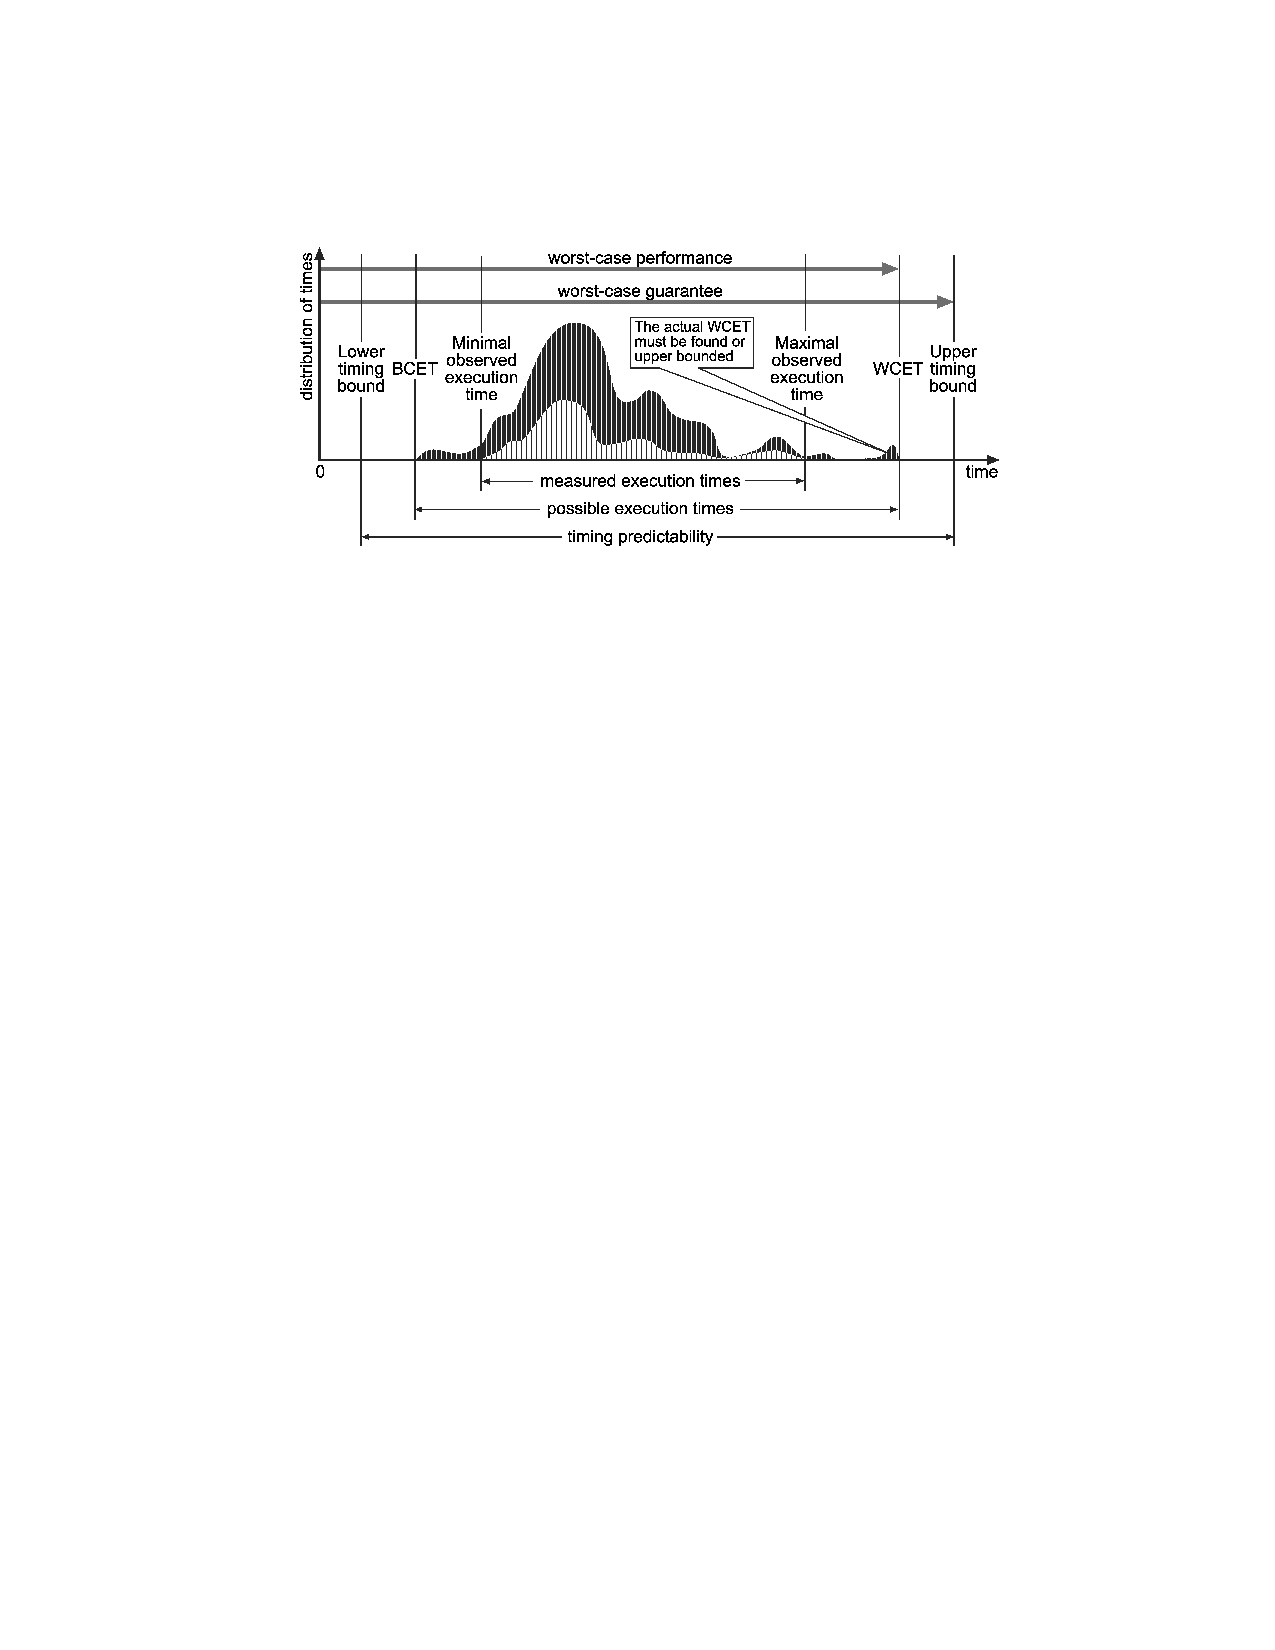
\includegraphics{figs/program_executiontimes.pdf}
  \end{center}
  \vspace{-3mm}
  \caption{``Program Execution Times~\cite{wilhelm-survey-paper}''}
  \label{fig:program_execution_times}
\end{figure}
It highlights several key issues that are important to understanding program execution time.
First, the \emph{observable execution times} may not observe all \emph{possible execution times}.
This is important because far too often we rely on testing and end-to-end measurement to determine the WCET.
This will, in general, overestimate the best-case execution time (BCET) and underestimate the WCET, and is not safe when timing must be guaranteed. 
Second, it is often difficult to determine the \emph{actual} WCET, thus the worst case guarantee that is given is usually a bound on the WCET.    
The goal of the WCET analysis is to obtain a \textit{safe} and \textit{precise} bound on the WCET of a program~\cite{wilhelm-survey-paper}. 
\textit{Safe} means that the execution time will never exceed the bounded time. 
\textit{Precise} means that the bounded time is as close to the absolute WCET as possible. 

Several factors contribute to the difficulties of a safe and precise WCET analysis.
In general, it is impossible to obtain the upper bounds on execution times for programs because programs are not guaranteed to terminate.  
Real-time systems use a restricted form of programming to ensure an execution time upper bound.
Recursion is often not allowed or must be explicitly bounded, as are the iteration counts of loops. 
Despite that, algorithms contain input dependent program paths that complicate analysis.    
The worst case program path depends on the worst-case input, which in general, is not known or hard to derive.    

Along with complications from the software structure, the execution time variance exhibited by the underlying architecture further complicates analysis.   
A conventional microprocessor executes a sequence of instructions from an instruction set. 
Each instruction in the instruction set changes the state of the processor in a well-defined way.
The microprocessor provides a strong guarantee about this behavior: a sequence of instructions \emph{always} changes the processor state in the sequential order of the instructions.        
For speed, however, modern microprocessors rarely execute the instructions strictly in sequence. 
Instead, pipelines, caches, write buffers, and out-of-order execution reorder and overlap operations while preserving the illusion of sequential execution.  
This causes the execution time of even the same sequence of instructions to fluctuate, depending on the architecture's underlying execution of its instructions.
To illustrate this, we show in figure~\ref{fig:simple_code_timing_issues} a code segment with a simple control structure and a static loop bound.

%predictability -   
  % C code example
  % modern architecture improvements
\begin{wrapfigure}{r}{0.45\textwidth}
  \vspace{-20pt}
  \begin{center}
    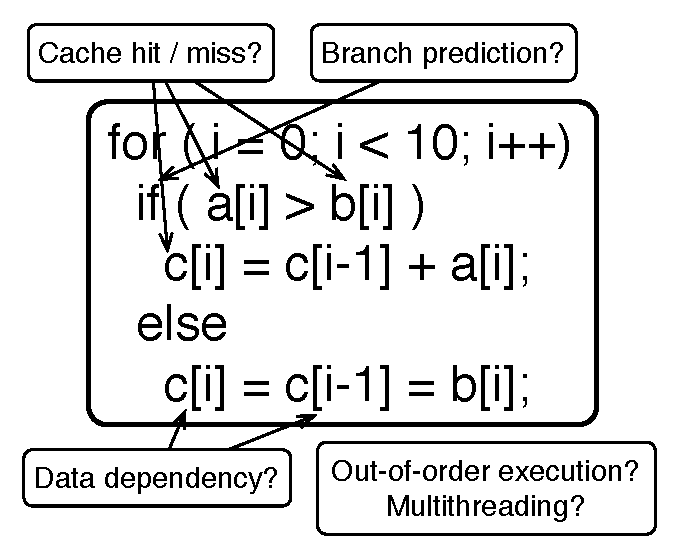
\includegraphics[scale=.6]{figs/simple_code_timing_issues}
  \end{center}
  \vspace{-10pt}
  \caption{Simple Loop Timing Issues}
  \label{fig:simple_code_timing_issues}
  \vspace{-10pt}
\end{wrapfigure}

Even with a simple software structure, several situations can arise from the execution on the underlying architecture. 
Each array access in the code is compiled into a memory access.
Whether the memory access hits or misses the cache has huge implications on program execution time.
The \emph{if} statement is usually compiled to a conditional branch.
The outcome of the branch predictor could easily affect the execution time of the program.
%Furthermore, the speculatively executed instructions could modify the cache state which can cause future memory accesses to delay.        
Superscalar architectures can execute instructions out-of-order, so data-dependencies in this code may or may not stall, depending on the memory accesses and how much loop unrolling is done by the compiler/architecture.   

Further complications arise as architectures become increasingly parallel with multiprocessing techniques such as multicore and multithreading.
These techniques allow the architecture to inherently handle concurrency, but can easily introduce temporal interference even between logically independent behaviors.
For example, in a multicore machine with shared caches, the processes running on one core can affect the timing of processes on another core even when there is no communication between these processes.
Similarly, Simultaneous Multithreading ~\cite{Tullsen1995SMT} architectures share a wide-issue superscalar pipeline across multiple hardware threads.
Instructions are dispatched from all threads simultaneously using scoreboaring mechanisms.
However, the contention for pipeline resources between threads can easily vary the execution time of a particular thread. 

% On the other hand, symmetric multiprocessing (SMP) techniques use multiple processing units connected with an on-chip communication interconnect such as a bus or network-on-chip.
% SMP exploits thread-level parallelism by designating a thread to a different processing unit.
% While this removes temporal interference caused by sharing pipeline resources between multiple threads, temporal interference is reintroduced at the on-chip communication interconnect.
% For instance, sharing the same off-chip memory between processing units requires arbitration and coherence, which results in temporal interference.
% In fact, any sharing of resources such as busses, memories, switches, buffers, and I/O devices can result in temporal interference.
\begin{wrapfigure}{r}{0.5\textwidth}
  \vspace{-20pt}
  \begin{center}
    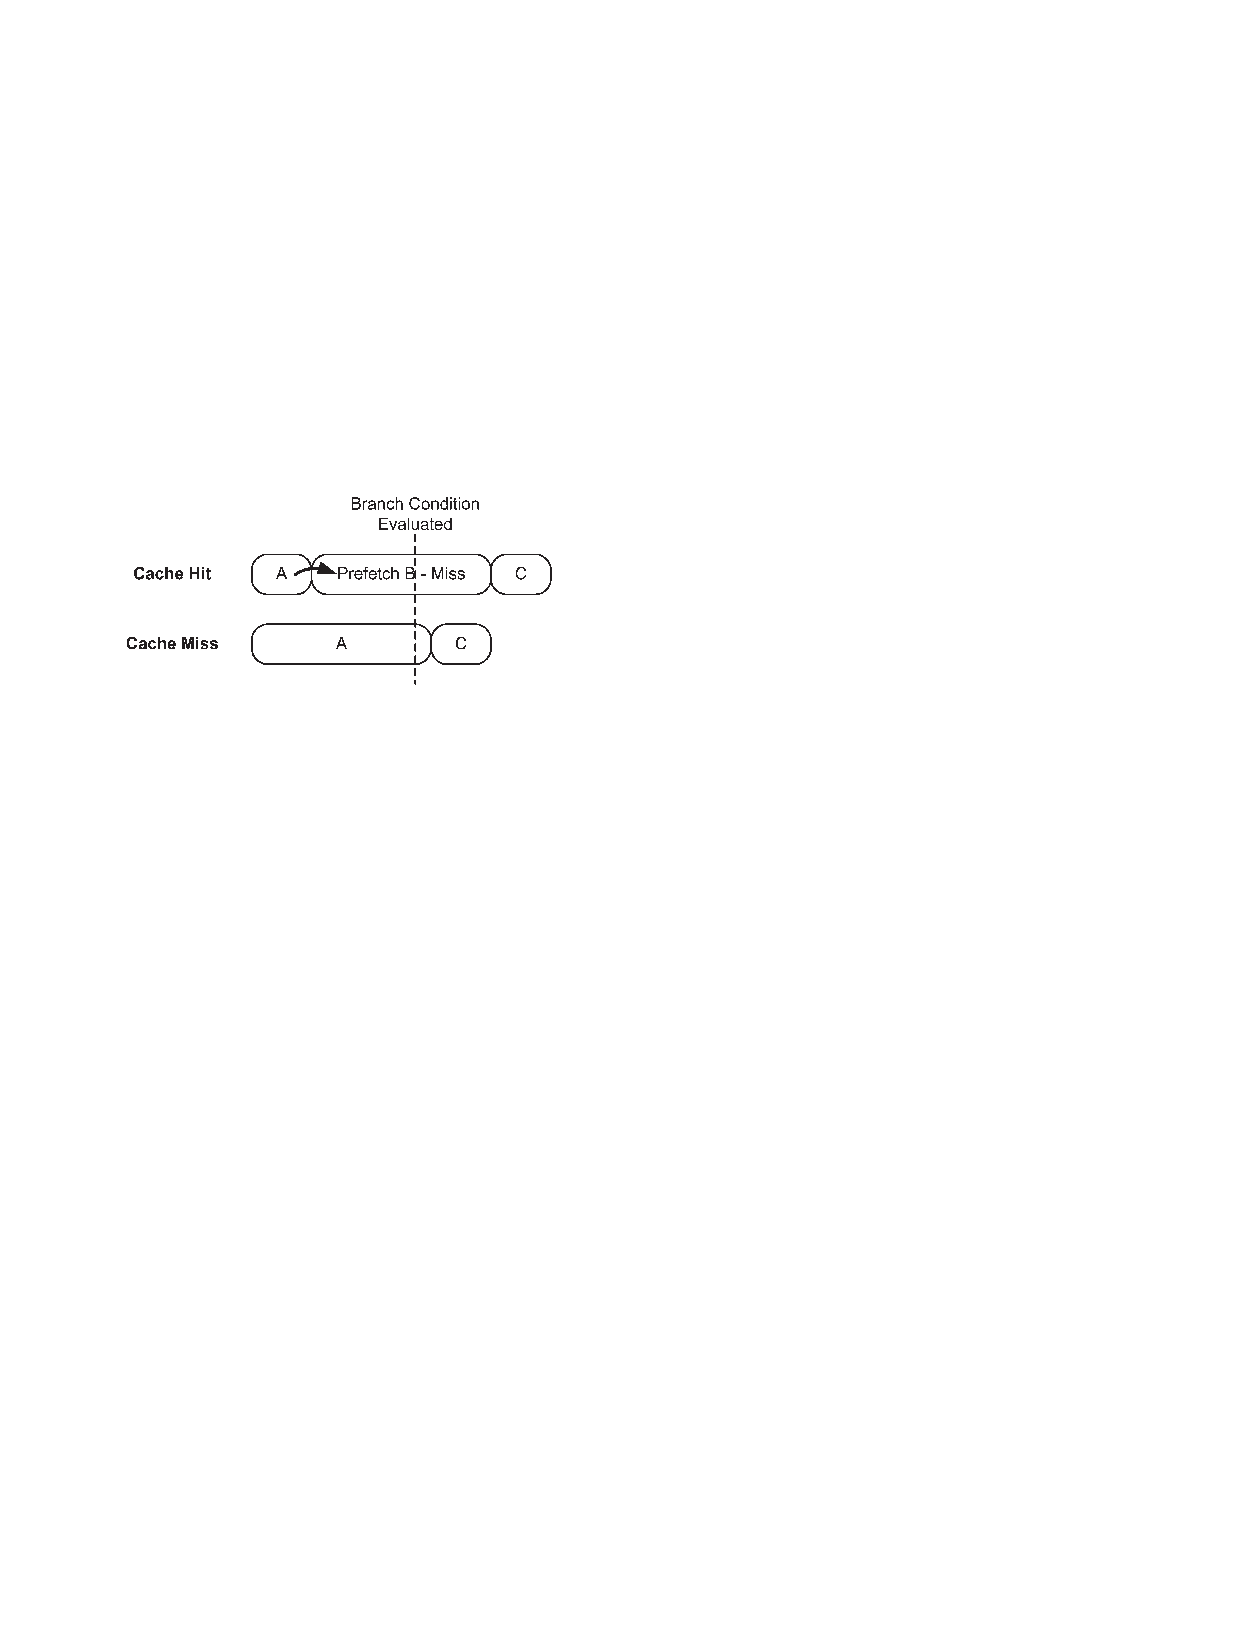
\includegraphics{figs/speculation_anomaly}
  \end{center}
  \vspace{-10pt}
  \caption{Timing anomaly cause by speculation~\cite{Reineke06adefinition}}
  \label{fig:speculation_anomaly}
  \vspace{-10pt}
\end{wrapfigure}
The common misconception is that at least a \emph{safe} upper bound on the execution time can be easily determined by assuming the worse case in unknown situations.
This is not true because dynamic processors can exhibit \emph{timing anomalies}~\cite{Reineke06adefinition,Lundqvist1999}; situations where a local worst-case does not result in the global worst-case.
Reineke et al.~\cite{Reineke06adefinition} illustrate this with the example shown in figure~\ref{fig:speculation_anomaly}.
In this example, a mispredicted branch results in unnecessary instruction fetching that destroys the cache state. 
However, if the first instruction being fetched is a cache miss, the correct branch condition will be computed before the fetch, and no speculatively executed instruction will destroy the cache state. 
This example shows that simply assume a cache miss (local worst-case) will not always lead to the global worst-case execution time.    

The increasing complexity of architectures leads to the conclusion that the usefulness of the results of WCET analysis strongly depends on the architecture of the employed processor~\cite{Heckmann2003processor}.
Modern processors employ features that improve average performance at the expense of worst-case performance, creating a large variation in execution time from the processor. 
These features are controlled and manage completely in hardware, not explicitly exposed to the software.
As a result, decrypting the state of the processor to obtain reasonable execution time estimates is often extremely difficult, if not impossible, on modern architectures.   

\section{Precision Timed Machines}
% As Wilhelm et al. \cite{Wilhelm_future_arch_09} quoted:
% \begin{quote} \textit{
%   ``The applicability of the AUTOSAR idea depends on availability of
%   architectures on which software composition does not lead to
%   unpredictable timing behavior.''
% }
% \end{quote}
In this thesis we present the design and implementation of a Precision Timed (PRET) machine~\cite{edwards2007case} -- the Precision Timed ARM (PTARM).
PTARM employs a thread-interleaved pipeline and a memory controller designed for predictable and composable execution.
It also implements an extended ARM~\cite{armrefman} ISA to demonstrate the ISA extensions with temporal semantics.
Our benchmarks show that an architecture designed for timing predictability and composability does not need to sacrifice performance.
%, and provides a robust, non brittle foundation for future cyber-physical systems.       

Many people have contributed to the results given in this thesis. 
The predictable DRAM controller that is presented in section~\ref{sec:pret_dram_controller} is a collaborative effort jointly done with Jan Reineke and Sungjun Kim. 
Hiren Patel, Ben Lickly, Jan Reineke, David Broman and Edward Lee have all greatly contributed to timing extensions to the ISA presented in section~\ref{sec:programming_models}.
And finally, the engine fuel rail simulation application presented in section~\ref{sec:1dCFD} is a collaborated effort with Matthew Viele, Guoqiang Wang and Hugo Andrade.
It is a pleasure to thank those who made this thesis possible, as this thesis could not have been complete without them. 
 
% In the remaining chapters we first discuss the design decisions of the hardware and ISA extensions in chapter~\ref{chapter:pret}, then show the details and architecture of PTARM in chapter~\ref{chapter:ptarm}.
% In chapter~\ref{chapter:app} we present two applications implemented with the PRET machine to demonstrate its applicability.
% Finally, in chapter~\ref{chapter:related} we discuss the related research work, and conclude in chapter~\ref{chapter:summary}.

% The remaining chapters are organized as follows. 
% Chapter~\ref{chapter:pret} explains the architecture of PRET including the \thdint pipeline and memory hierarchy, Chapter~\ref{chapter:ptarm}, Chapter~\ref{chapter:app}, Chapter~\ref{chapter:related}, Chapter~\ref{chapter:summary}.

%We aim to present architectures
%proposed a paradigm shift in the design of computer architectures, focusing on timing predictability instead of average-case performance.
%provide better wcet
%use thread-interleaved pipline and dram controller
%ISA extensions
%needed for autosar etc




% \begin{itemize}
% \item \emph{Low jitter} -- Small variance in execution time for a given code block, enabling a tight WCET bound.
% \item \emph{Continuous}~\cite{Henzinger2008} -- small changes in the input result in small changes in the output.
% \item Precise timing control, which is the ability to control temporal
%   properties in the architecture.
% \item Reasonable performance, or else someone could use a processor
%   from 20 years ago to achieve some of the effects above.
% \item Repeatable performance, mainly that the same execution yields
%   the same output. Including execution time. (\textcolor{red}{This
%     needs careful defining... what counts as input and what counts as
%     output?})
% \item Composability - The ability to compose two tasks without
%   interference. This is an extremely important property to preserve
%   because when we design systems, we want to design larger systems
%   from smaller components. We want to test those smaller systems
%   separately, then compose them and still have those tested properties
%   hold true. 
% \end{itemize}
% Through this, enable evaluation on the effects and implications on the composition, communication and synchronization of software components or tasks on a predictable architecture.





\chapter{Related Work}
\label{chapter:related}
\label{sec:related_arch_mod}
We are certainly not the first or only one to tackle the unpredictability of computer architecture designs.
In this chapter we survey an abundance of related research to our goal of predictable architectures.
Timing analysis techniques, compiler techniques and architectural techniques all play a role in tackling the unpredictability of computer architectures.
However, we limit the scope of this survey to mainly focus on architectural techniques, as that is the focus of this thesis. 
Adding temporal semantics to programming languages has been the focus of many research proposals, but to the best of our knowledge, we believe this is the first attempt to introduce temporal semantics down at the ISA level. 

%FIXME: Compare to XMOS style handling of interrupts?

\section{Pipeline-Focused Techniques}
\subsection{Static Branch Predictors}
\label{sec:RTBranch}
Dynamic branch predictors cause timing anomalies~\cite{Engblom2003dynbranch}, and they are difficult to model because of the \textit{aliasing} of branch points.   
\textit{Aliasing} occurs when two different branches occupy the same branch predictor slot and cause interference.
Burguiere et al.~\cite{Burguiere2005staticbranchpredict} make a case for \textit{static branch prediction} to be used for real-time systems.
This can be done in several ways. 
The simplest form can predict all branches taken or not taken. 
Improvements can include the \textit{Backward Taken, Forward Not Taken} scheme, to improve performance for loops and if statements.
This scheme uses the observation that for loop control branches, almost all backwards branches are taken to return to the loop; only at the end of the loop are forward branches taken. 
With architecture support for static branch predictions, compilers can analyze code patterns (loops, if-then-else, if then) and insert instruction set constructs to denote the static prediction of each branch.  
The underlying architecture will use that for its prediction, instead of relying on a dynamic hardware unit.
This removes \textit{aliasing} and gives better estimated worst case branch mispredicts. 

Bodin et al.~\cite{Bodin2005staticbranch} use this idea of software static branch prediction to improve the WCET of programs.
Intuitively, they aim to remove all branch mispredict penalties from the worst-case path to improve the WCET. 
They propose an algorithm that iterates through the control flow graph to find the worst-case execution path (WCEP). 
Initially, the algorithm finds the worst case path assuming all the branches are mispredicted. 
Then, the algorithm assigns the static branch prediction of all branches on the WCEP to be taken.
The algorithm then iterates again to find the new WCEP until two iterations yield the same WCEP.
Since the algorithm never reassigns assigned branches, it always converges but is not optimal.
The presence of caches can easily effect the WCEP, and each branch prediction reassigned can modify the cache state.
However, the experiments assumed all code and data fit into the caches, thus the effects of caches were not factored into the algorithm.

\subsection{Superscalar Pipelines}
\label{sec:RTSuperscale}
Superscalar pipelines issue multiple instructions at a time to exploit instruction-level parallelism (ILP). 
In order to keep the pipeline filled, superscalar pipelines typically employ more aggressive techniques to fully utilize the ILP. 
As a result, attempting to model all advanced techniques often leads to either very pessimistic results, or almost infeasible complex models.

Rochange et al.~\cite{Rochange2005superscalar} propose to use instruction pre-scheduling to ease the difficulties of analysis of superscalar pipelines.  
The concept is similar to resetting the pipeline state before each basic block execution. 
This is done by postponing the scheduling of instructions from the next basic block until the instructions from the previous basic block are completed.
If it is possible to remove all timing interference across basic blocks, then the resources needed to model the pipeline can be significantly reduced, as each basic block will start with a consistent initial state.
However, the results assume the absence of caches, which can easily effect execution across basic blocks.  
Furthermore, depending on how many instructions can be in flight at one time, waiting for the pipeline state to be flushed can induce large penalties for programs with a lot of control flow transfer and small basic blocks. 

% \paragraph{A time-predictable execution mode for superscalar pipelines with instruction prescheduling ~\cite{Rochange2005superscalar}}
% \begin{itemize}
% \item What is the background of this work? What is the motivation?\\
% 
% \item What is the main goal?\\
%   They want to reconcile high performance with time
%   predictability. Mainly, they are making out of order superscalar
%   pipelines fit WCET estimation techniques. 
% \item What did they do to achieve this goal?\\
%   They control instruction flow to remove dependence between basic
%   blocks so that any WCET estimation tool would only need to measure
%   or estimate a smaller segment of code.  
% \item How do they evaluate their approach? Does it achieve the goal?
%   Do they compare it with other work?\\
%   They showed a performance comparison of slow down compared to
%   regular out of order superscalar and also against in order scalar
%   pipeline to show performance improvement. 
% \item What other work is listed as future work?\\
% \end{itemize}
% Additional questions:
% \begin{itemize}
%   \item What are the limitations/assumptions of this work?\\
%     They ignore peripheral components (cache memories, TLBs) as well
%     as external events (interrupts) and interactions with the
%     operating system (process scheduling, virtual memory, etc).
%   \item Which parts of a system/design process are modified by this
%     work? (e.g. hardware (which feature?), WCET analysis, scheduling,
%     compiler, programming language, \ldots)\\
% \end{itemize}


% \paragraph{Predictable Out-of-order Execution Using Virtual Traces ~\cite{whitham:08:predOOOwithVirtualTraces}}
% \begin{itemize}
% \item What is the background of this work? What is the motivation?\\
%   The motivation is to improve WCET of complex processors,
%   specifically for out-of-order superscalar pipelines. 
% \item What is the main goal?\\
%   The main goal of this paper is 3 fold. 1) minimizing the pessimism
%   introduced in WCET analysis. 2) increasing CPU throughput that can
%   be guaranteed. 3) minimize CPU modeling cost. 
% \item What did they do to achieve this goal?\\
%   They introduced a VTC (virtual trace controller) to control the
%   progress of the pipeline. They argue that this controller can be
%   used for a CPU of arbitrary complexity. The VTC operates CPU
%   programs as a collection of traces. Traces are paths through the
%   program. Essentially traces are formed by statically predicting
%   branches, in the context of this paper they predict the branches
%   towards the worst case execution path. This way the pipeline
%   optimizations (out of order execution etc) can optimize the worst
%   case path. This achieves goal 2, which is increased the guaranteed
%   throughput. The traces are formed via static branch predictions, and
%   the VTC contains a VTR (virtual trace register) which stores the
%   branch predictions. The pipeline state is reset between traces, so
%   the WCET analysis can be limited to within traces. The side exits
%   are determined by branch mispredicts. Now WCET within each trace and
%   side exit can be measured, and it will be the same execution time,
%   thus no CPU modeling cost is needed. This achieves goals 1 and 3. 
% \item How do they evaluate their approach? Does it achieve the goal?
%   They use the Malardalen WCET benchmark suite, but assume that
%   benchmark programs are single-path programs. They assume using IPET
%   or methods can find the WCET. They use the benchmark programs and
%   run the program on an idealized in order machine to compare the
%   results with their machine. They compare the speed up /slow down and
%   use it to analyze the issues with their approach. 
% \item What other work is listed as future work?\\
% \end{itemize}
% Additional questions:
% \begin{itemize}
%   \item What are the limitations/assumptions of this work?\\
%     They assume WCEP is easily obtained. It also depends on how many
%     traces are formed, and how effective the traces are formed. They
%     assume scratchpads in this work.
%   \item Which parts of a system/design process are modified by this
%     work? (e.g. hardware (which feature?), WCET analysis, scheduling,
%     compiler, programming language, \ldots)\\
%     They need a compiler to compile code into traces and form
%     traces. The hardware is modified with a VTC to control the traces
%     and stall the pipeline between traces. 
% \end{itemize}


Whitham et al. \cite{whitham:08:predOOOwithVirtualTraces} combine the techniques of instruction pre-scheduling and static branch predictions to propose modifications to an out-of-order superscalar pipeline to provide predictability for single thread execution.  
Instead of basic blocks, the superscalar pipeline pre-schedules instructions across \emph{virtual traces}\cite{Whitham2008formvirtualtraces}. 
\emph{Virtual traces} are program paths with static branch predictions inserted. 
These are usually formed by predicting along the WCEP, similar to the algorithm introduced by Bodin et al~\cite{Bodin2005staticbranch}. 
Each virtual trace can contain a fixed number of branches. 
A VTC (virtual trace controller) is introduced to control the progress of the pipeline.
The VTC contains a VTR (virtual trace register) which stores the branch predictions.
The pipeline state is reset between traces so the WCET analysis can be limited to within traces.
The out-of-order superscalar pipeline is also modified to disallow memory prediction and reordering of branches.
The architecture employs scratchpads instead of caches.  
This allows the execution of traces to run predictably for each different exit (branch mispredict) within a trace.
The architecture shows an improved throughput for most programs when compared to a simple in-order CPU model.
%The authors further present the effects of trace sizes to balance the main path execution time against the costs of side exits. 

% There are issues with this work, as the assumption is the ability to find the WCEP when doing the trace scheduling (how do you obtain numbers for the basic blocks with Out of Order execution, and what if program itself is so complex that the analysis is nearly infeasible?). 
% But the idea of using static branch prediction in combination with WCET could be leveraged. 
% The delayed scheduling of traces to flush the pipeline could be a huge penalty for programs with small tasks that execute frequently. 
% Reducing this delay is thus a trade off between performance of traces vs amount of state to keep to obtain the performance.

\subsection{VLIW architectures}
\label{sec:RTVLIW}
VLIW machines, like superscalars, issue multiple instructions at a time to exploit ILP.
However, unlike superscalars, VLIW machines rely on the compiler to utilize ILP and determine the instructions issued.  
This helps in the predictability because the hardware does almost no reordering or stalling.
 
Yan et al.~\cite{Yan2008VLIW} study the predictability of VLIW machines, and propose changes to the architecture and compiler to improve the predictability. 
They find that although most of the data dependency is scheduled away by the compiler, there are still several factors that limit the predictability on the hardware. 
First, since statically it is not known whether a memory access is a hit or a miss, the hardware still needs to check for it and stall when needed. 
Second, data dependencies still exist across compilation units, so the hardware still needs to support basic data dependency checking to handle those dependencies.
A compilation unit could be a basic block, a loop, a procedure or a region~\cite{Hank:1995:RCI:225160.225189}. 
Finally, if the VLIW machine uses branch prediction, there is still the need for the handling of mispredictions.

As VLIW machines heavily utilize the compiler to improve performance, they propose several compiler techniques to compile programs that lend themselves to better WCET. 
First, they use the single-path paradigm proposed by Puschner and Burns~\cite{Puschner:2002:WTP:882515.885528}, and eliminate all non-loop backwards branches with full if-conversions~\cite{Allen:1983:CCD:567067.567085}.  
To mitigate the performance penalty of single-path programming, aggressive hyperblock scheduling~\cite{Mahlke:1992:ECS:144953.144998} is used to exploit the ILP from VLIW architectures. 
For the data dependencies across compilation units, they use code padding to ensure the execution time is consistent across different paths.    
This will enable easier WCET analysis. 
This work minimally deals with instruction caches, but does not account for the effects of data cache. 

\subsection{Multithreaded Pipelines}
\subsubsection{Thread Scheduling}
With explicit hardware multithreading, the scheduling policy plays a huge role in the predictability of the architecture.
Kreuzinger et al.~\cite{Kreuzinger2000RTmultithread} evaluate the use of different real time scheduling schemes to schedule hardware threads to handle external events. 
They evaluate fixed priority preemptive (FPP), earliest deadline first (EDF), least laxity first (LLF) and guaranteed percentage (GP), which is similar to time sharing the pipeline. 
The architecture used for evaluation is a Java multi-threaded superscalar pipeline with four threads~\cite{Kreuzinger2003multithreadeventhandle}. 
A hardware priority manager is implemented to facilitate the scheduling of threads. 
All real-time threads register their real-time requirements during initialization with the priority manager. 
When the external event occurs, the priority manager schedules the corresponding interrupt service thread, and starts assigning priorities based upon the real time requirements. 
The evaluation criteria to compare scheduling policies is the throughput of the processor. 
The conclusion of the report is that in order to maximize multiple threads on a superscalar machine, the scheduler should try to keep as many threads active as long as possible to leverage thread level parallelism and hide more latencies of pipeline stalls. 
Thus GP does the best because it schedules different active threads each cycle until their percentage runs out.
Thus, it keeps threads alive as long as possible. 
The idea of using hardware threads to service interrupts is novel because of the low overhead to switch contexts. 
By giving the interrupt service routine thread priorities, it may be possible the bound the execution time of higher priority threads. 
Although the dynamic thread scheduling can cause execution time bounds to be imprecise from the effects of timing interference across threads.  
  
El-Haj-Mahmoud et al.~\cite{El-Haj-Mahmoud2005VirtualMultiprocessor} propose a statically scheduled multithreaded architecture called the Real-Time Virtual Multiprocessor (RVMP).   
The idea of a virtual processor is a slice of time on the processor. 
The RVMP extends an in-order 4-way superscalar processor to support the partitioning of the pipeline in \emph{space} and \emph{time}.  
In the \emph{space} dimension, the resources of the superscalar can be partitioned to different threads. 
In the \emph{time} dimension, the superscalar resources are time shared, and different threads are scheduled to utilize the resources at different times.  
The hardware extensions to the superscalar pipeline prevent interference between the virtual partitionings.
Scratchpads are employed for predictable memory access latencies, although they assume all accesses go to the scratchpad. 
It is unclear how accesses to shared resources, in particular main memory are dealt with.
A static round-based schedule of the thread execution is constructed to account for the real-time requirements of each thread.
The static schedule utilizes the flexibility of the different time and space partitioning options to allow threads with higher utilization more access to the pipeline. 

\subsubsection{Simultaneous Multithreaded Architectures} 
\label{sec:RTSMT}
Simultaneous Multithreaded Architectures (SMT) attempt to exploit both instruction-level and thread-level parallelism by dynamically scheduling multiple hardware threads onto a multi-way pipeline. 
In each cycle, instructions from different threads can be fetched simultaneously to fully utilize the pipeline.
The dynamic scheduling and aggressive speculation techniques render SMTs almost impossible to use for real-time systems.  
However, several proposals involve slight modifications to architecture to create a \emph{WCET-aware} SMT to be used for real-time systems.  

Barre et al.~\cite{Barre2008RTSMT} propose to assign one explicit hardware thread with the highest priority. 
That thread, called the real-time thread, gains access to any resource whenever it is scheduled. 
Any other thread that is currently occupying the resource will be preempted, and later replayed when the real-time thread is not using it.
The modifications to the SMT include additions to allow the preemption, and also the partitioning of any resource that needs to be shared. 
This gives the highest priority thread the illusion that it has the whole superscalar pipeline to itself, reducing the execution time analysis of the real-time thread to the equivalent of a superscalar architecture. 
Currently the cache effects and branch prediction are listed as future work.  

Hily et al.~\cite{Hily1999} show that out-of-order execution may not be as cost effective as in-order execution on SMT machines.
Thus, Uhrig et al.~\cite{SaschaUhrig2005SMT} propose a similar concept to Barre et al.~\cite{Barre2008RTSMT}, except for an in-order executed superscalar.
Mische et al.\cite{Mische2008SMT} expand this to allow more than one real-time thread to run on the SMT architecture.
This is done by time-sharing the highest priority thread slot among the real-time threads.  
The time-sharing schedule is statically constructed to ensure that the real-time threads still provide reasonable WCET guarantees. 
This architecture uses instruction scratchpads without data scratchpads, and no branch predictors, as the branch penalty can be filled with executions from other threads.   
Some issues do arise with the contention of memory access, as it is difficult to partition memory accesses between hardware threads.
Contention between the high priority thread slot and other thread slots are resolved by alerting the memory controller from earlier stages in the pipeline that a high priority thread will issue a memory instruction. 
This way the memory controller can hold off service to the lower priority memory accesses and wait for the high priority access to come.     
However, it is unclear how contention between the real-time threads on the high priority thread slot is resolved.
 
% \bigskip
% Although real time SMT proposals have a lot of compelling features, it
% still lacks a formal WCET analysis. All of the proposals have just
% used measured benchmarks to prove performance, and assumed that
% because the high priority thread runs as if no other thread is
% running, so static analysis is possible. In reality, WCET for a
% superscalar processor already contains pessimistic results. Although
% the lack of a branch predictor and in order execution may aid in
% this. Also, in this line of work still only one explicit hardware
% thread slot gets real-time performance, while the other threads'
% performance will have a non-continuous penalty, which is hard to
% categorize. 

\subsubsection{Thread Interleaved Pipelines}
Thread-interleaved pipelines have been proposed and employed in various architectures from research and industry. 
Besides the CDC6600~\cite{CDC6600}, described in section~\ref{section:pret_thread_pipeline}, Lee and Messerschmitt~\cite{lee1987pip}, the Denelcore HEP~\cite{HEP}, the XMOS XS1 architecture~\cite{xmos_xs1}, the Parallex Propeller chip~\cite{parallex} and the Sandbridge Sandblaster~\cite{Erdem02multi-threadedprocessor} all use fine grained thread interleaving for different applications. 
In particular, Lee and Messerschmitt~\cite{lee1987pip} and the Sandbridge Sandblaster~\cite{Erdem02multi-threadedprocessor} propose the use of thread-interleaved pipelines for DSP applications. Lee and Messerschmitt~\cite{lee1987pip} also use a round robin thread scheduling policy while the Sandblaster uses a Token Triggered Threading policy. 
The Token Triggered Threading policy is similar to the round robin scheduling policy in that each hardware thread context can only issue one instruction each in a scheduling cycle. 
However, a token is used to determine which thread's instruction is executed next. 
The XMOS XS1 architecture~\cite{xmos_xs1} allows hardware threads to dynamically be added and removed from the thread scheduling.
They use the dynamically added threads to handle interrupts, which improves the interrupt response latency. 
The XS1 architecture specifies that during execution, there will always be a minimum the number of threads equal to the pipeline depth. 
As explained in section~\ref{section:pret_thread_pipeline}, this removes pipeline hazards to improve throughput.
However, the dynamic thread scheduling can cause each thread's execution frequency to vary depending on the number of threads executing at one time.         

\subsection{Others}
\subsubsection{Virtual Simple Architecture}
Anantaraman et al.~\cite{Anantaraman2003VISA} propose the virtual simple architecture (VISA), which uses dynamic checking to ensure tasks are meeting the deadlines. 
The microarchitecture is split into two modes. 
A simple mode, which conforms to the timing of a hypothetical simple pipeline that is amenable to safe and tight WCET analysis. 
And a high performance mode, in which the architecture can use arbitrary performance-enhancing features.
A task that executes on the VISA is divided into multiple sub-tasks to gauge progress on the complex pipeline.
Each sub-task is assigned an interim deadline, based on the hypothetical simple pipeline.  
When tasks are executing on the VISA, they are first speculatively executed in high-performance mode.
If no checkpoints are missed, then the high performance mode has met the timing requirements. 
If a checkpoint is missed, the architectures switches to a simple mode to bound the remaining task times in attempt to meet the timing constraints.
The results show that the high performance mode have average executions times of 3 to 4 times faster than the simple mode.
The authors also discuss possible power savings by scaling the voltage in high performance mode.
However, the tasks and programs must have sufficient slack time to allow for dynamic checking of deadlines, and it is unclear whether the simple mode will always be able to make up the time if the high performance mode misses its checkpoint. 

\subsubsection{Java Optimized Processor}
\label{sec:RTJava}
Schoeberl presents the Java Optimized Processor (JOP)~\cite{jop:wcet} which uses Java for real time embedded systems. 
The design of JOP includes a two level stack cache architecture ~\cite{jop:stack}. 
Instead of using a large register file to store the stack, like the PicoJava\cite{McGhan1998PicoJava}, it uses only two registers to store the top two entries of the stack (Register A and Register B). 
Leveraging the stack based architecture of JavaVM, whenever an arithmetic operation occurs, the result is always stored back to the top of the stack (Register A). 
Any push or pop operation simply results in a shift of values between the two registers and the stack cache, which only requires one read and one write port for the memory. 
This architecture does not have any data hazards and has very few pipeline stages (no need for an explicit commit/writeback stage). 
Because of the few pipeline stages, it only has a small branch delay penalty, so no branch predictor is used.
All bytecode on JOP is translated into a fixed length microcode. 
Each microcode executes in a fixed number of cycles, independent of its surrounding instruction.
Thus, the WCET analysis only requires a lookup table of bytecode translated into microcode, rendering it a predictable architecture. 

\subsubsection{MCGREP}
Whitham introduces the Microprogrammed Coarse Grained Reconfigurable Processor (MCGREP)~\cite{whitam:06:mcgrep}, which is a reconfigurable predictable architecture.
The architecture of MCGREP contains multiple execution units, but each operation is implemented in microcode. 
The pipeline architecture is extremely simple, reassembling a two stage pipeline with a fetch/decode stage and an execute stage.
No internal state is stored in the pipeline, and instructions do not affect each other's execution time. 
A fast internal RAM without cache is used to store the program and used as memory for data.    
The microcode operations are predictable in the MCGREP architecture, taking a fixed number of cycles to complete.
Advanced operations can be dynamically loaded as new microcode, which enables application specific instructions to improve performance.
All MCGREP instructions take a fixed number of clock cycles to complete and are unaffected by execution history, making MCGREP a predictable processor. 

\subsubsection{ARPRET}
Andalam et al.~\cite{pretc} introduce the Auckland Reactive PRET (ARPRET) architecture to execute a new language called precision timed C (PRET-C).
PRET-C is a synchronous language extension to C designed to support synchronous concurrency, preemption, and a high-level construct for logical time.
ARPRET extends the Microblaze~\cite{xilinx-microblaze} with a custom Predictable Functional Unit (PFU) that is used for thread scheduling.
The Microblaze is configured to use on-chip memory to achieve predictable memory access latencies. 
The PFU stores the thread contexts of each thread, including the PC, thread status, priority, etc. that are used during each context switch.
By doing the thread scheduling in hardware, ARPRET reduces the thread switching overhead. 
Each thread switch is triggered in software by the C language extensions in PRET-C, and the PFU is used to determine the next context to run.   
Their benchmarks show that the ARPRET achieves predictable execution without sacrificing throughput. 
% \subsubsection{PRET}
% Craven et. al~\cite{Craven_PRET_implementation_2010}  implements PRET thread interleaved pipeline as an open source core using OpenFire 

\section{Memory-Focused Techniques}
\subsection{Caches}
The dynamic behavior of caches cause headaches for real-time systems when trying to predict memory access latencies.
Reineke et al.~\cite{Reineke07TimingPredictability} presented a study on the predictability of different cache replacement policies.
They evaluate the Least Recently Used (LRU), First In First Out (FIFO), Pseudo LRU (PLRU) and Most Recently Used (MRU) replacement policies to determine if LRU was more predictable than other policies, as observed by Heckmann et al.~\cite{Heckmann2003processor}.    
The results confirm that the LRU replacement policy was significantly more predictable than other policies.
Thus, the authors recommend any real-time system with caches to use LRU for its replacement policy. 
This paper also reveals potential for improvement in existing analyses of PLRU and FIFO.

Puat and Decotigny~\cite{Puaut02} propose to use partitioned and lock caches to eliminate the intra- and inter-task interferences when a cache is used. 
Intra-task interferences occur when different memory blocks of the same task compete for cache blocks.
Inter-task interferences occur when a preempting task's memory blocks cause cache reloads in the preempted task.
By using cache partitioning, a part of the cache is reserved for a particular task, and inter-task interference is eliminated.
To eliminate intra-task interference, cache locking is used to lock the contents of cache.
The cache contents can be locked statically, which are fixed at system start for the whole run time, or dynamically, where the contents may change.   
By locking and partitioning caches, the memory access latencies will have more predictable behavior. 

Schoeberl~\cite{jop:jtres_cache} propose to use method caches for the instruction cache of the JOP architecture~\cite{jop:wcet}.
Conventional caches use a cache line as its basic unit of replacement. 
Method caches use \emph{methods} as its unit of replacement. 
A cache can contain different block sizes that are used to store methods. 
There exists a tradeoff between performance and predictability for the block sizes of the method cache. 
Methods can occupy more than one block, depending on the method size. 
When a method is called, the cache loads the whole method into the cache, occupying any number of blocks it needs.
The LRU replacement policy is used, since the end of a method usually returns to its parent method. 
When a method is evicted, all blocks it occupies are evicted. 
Thus, the instruction cache is more predictable, because it only changes on method calls. 
Within a method, all instructions are known to be in the cache, so no cache miss results from the instruction cache.
 
%method cache SMT
Metzlaff et al.~\cite{Metzlaff2008MethodcacheSMIT} use a method cache mechanism with the real-time SMT architecture in ~\cite{Mische2008SMT}.
They partition the scratchpad for each different thread so no inter-thread interference will exist.   
Then, they implement the method cache~\cite{Kirner2007ModelFunctionCache} with scratchpads, and give priority to the high priority thread when a filling is needed.
They called this the function scratchpad.  
If the thread is stalled when a method is being filled into the scratchpad, other threads occupy the pipeline, so throughput is preserved with multiple threads. 

\subsection{Scratchpads}
Scratchpads are known to allow more precise WCET analysis~\cite{Wehmeyer2005SPM} because the contents are managed in software. 
Puaut et al.~\cite{Puaut2007SPMvsCache} present a comparison of locked caches and scratchpads, and show only subtle differences between the two in terms of performance. 
Most benchmarks give similar WCET estimates. 
The difference stems from the granularity of allocation units. 
For locked caches, the basic allocation unit is a cache line. 
Thus, it is possible to \emph{pollute} the contents of the cache line with contents that are not part of the allocation scheme. 
Also, depending on the associativity of the cache, a cache line that should be locked could possibly be in conflict with another cache line that is also locked, and thus lose its ability to be locked in the cache. 
For scratchpads, the basic allocation unit is only determined by the allocation scheme, so the contents cannot be polluted. 
However, if the basic allocation block is big, it is possible that the allocation block will not fit in the scratchpad at the end due to fragmentation.  
 
% 
% \bigskip
% \textbf{Preemption} - Although scratchpads are more predictable, the
% hardware replacement policy of caches could be advantageous,
% especially for systems that have preemption of tasks. Locked caches
% can lock content in the cache, and when a preemption occurs, the
% hardware can still take advantage of a hardware replacement for lines
% that aren't locked, while still maintaining a certain amount of
% predictability when the original task resumes (because of the locked
% content that aren't replaced). For statically allocated scratchpads,
% the allocation scheme needs to take into account the preempted task,
% and allocate space for that task. This will reduce the available
% allocation space for all other tasks. For dynamically scheduled
% schemes, it will be extremely difficult to find reload points to
% adjust the scratchpad. If a preempted task loads its optimal content
% when it preempts a task, it's unclear what to load back for the
% original task, and when to load it. There needs to be some sort of OS
% that keeps track of what was loaded off the scratchpad. It is unclear
% what overhead this could result in. (\textcolor{red}{Read papers about
%   this} \JR{Write paper about how to do this ;-)})
% 

% Scratchpad (SPM) memories provide time-predictable accesses for data.  
% However, the time-predictable SPM allocation strategies for data only support statically allocated data or stack data.  
% Dynamic data, on the other hand, is only supported by non time-predictable allocation schemes if whole-program pointer analysis identifies every memory operation that could access each variable.
 
Whitham and Audsley~\cite{whitham:09:timepredLoadStore} introduce a hardware scratchpad memory management unit (SPMMU) that manages the transfers of data between memory and the data scratchpad to eliminate \emph{pointer aliasing} and \emph{pointer invalidation}.
\emph{Pointer aliasing} occurs when the same memory location is referenced using different names (pointers). 
\emph{Pointer invalidation} occurs when an object in a memory location is moved out from that memory location.  
As a result, an alias that points to the object before the move, ends up pointing to an incorrect object.
They propose to separate \emph{logical addresses} (used by the program) and \emph{physical addresses} (identifying where an object resides).  
The SPMMU maintains a table mapping the logical address and physical address.   
Although the SPMMU resides in hardware, its contents are controlled by software via explicit OPEN and CLOSE commands in the code.  
The user specifies the base address for the object, the size of the object and the physical address at which the object is being loaded to. 
The SMMU then performs the transfer, and updates an internal table mapping the logical address to the new physical location of the object.  
This simplifies analysis because it eliminates the need for whole-pointer analysis in the program. 

% \paragraph{Implementing Time-Predictable Load and Store Operations~\cite{whitham:09:timepredLoadStore} }
% 
% \begin{itemize}
% \item Basic definitions: \\
% \textbf{Pointer aliasing:} The same memory location may be referenced using different names (pointers). 
% \textbf{Pointer invalidation:} An object in a memory location is moved out from that memory location.  As a result, an alias that points to the object before the move, ends up pointing to an incorrect object. 
% \textbf{Whole-program Pointer analysis:} Determine which pointers can point to which variables and storage locations in the entire program.
% \item What is the background of this work? What is the motivation?\\
% Scratchpad (SPM) memories provide time-predictable accesses for data.  However, the time-predictable SPM allocation strategies for data only support statically allocated data or stack data.  Dynamic data, on the other hand, is only supported by non time-predictable allocation schemes if whole-program pointer analysis identifies every memory operation that could access each variable. 
% \item What is the main goal? \\
% The objective of this paper is to implement a scratchpad memory management unit that transfers data between external memory and scratchpad memories such that pointer aliasing and pointer invalidation are eliminated. 
% This approach lifts some of the restrictions (i.e. eliminate pointers entirely from program code or no support for dynamic data) forced by the limitations of WCET analysis. 
% \item What did they do to achieve this goal?\\
% They implemented a scratchpad memory management unit (SPMMU) in hardware that performs a mapping from logical addresses (used by the program) to physical addresses (identifying where an object resides).  In addition, the SPMMU performed DMA transfers between the external memory and SPM.  The program dictates when the transfers take place via explicit OPEN and CLOSE commands in the code. The user specifies the base address for the object, the size of the object and the physical address at which the object is being loaded to.  The SMMU then performs the transfer but updates an internal table mapping the logical address to the new physical location of the object.  
% \item How do they evaluate their approach? Does it achieve the goal? Do they compare it with other work?\\
% They use three approaches to evaluate their work.  
% Their first approach simply looks at the hardware cost incurred.  In particular, they observe that since the mapping must take place in the same cycle that the request is made, it must be implemented as combinational logic; hence, a part of the critical path.  They determine this critical path and its effect on the clock frequency. 
% The second approach compares their approach for a particular function of a JPEG decode algorithm with a data cache with estimated access latencies.  They show that the SMMU is not as effective as a data cache in ideal conditions, they are much better in the worst case. 
% The third approach is a case-study implementation of the entire JPEG decode algorithm with the SMMU. 
% \item What other work is listed as future work?
% Integrating one of the SPM allocation techniques with the SMMU to determine the where to place OPEN and CLOSE commands. 
% \end{itemize}
% Additional questions:
% \begin{itemize}
%   \item What are the limitations/assumptions of this work?\\
% The user must specify the size of the object and the physical address. 
% They claim that there are algorithms that determine the best physical address, but I haven't read that work yet. 
%   \item Which parts of a system/design process are modified by this work? (e.g. hardware (which feature?), WCET analysis, scheduling, compiler, programming language, \ldots)\\
% They require the following modifications: 1) hardware, 2) WCET analysis, and 3) compilers to generate the OPEN/CLOSE commands. 
% \end{itemize}

% \subsubsection{Static allocation schemes}
% \label{sec:SPM_static_allocation}
% Static allocation schemes allocate the content on the scratchpad a
% priori, and the content stays the same throughout the whole
% execution. Most static scratchpad allocation schemes
% (\textcolor{red}{Find some citations}) use some sort of heuristic to
% find the most commonly executed instructions or data structures, and
% then allocate them statically on the scratchpad to improve the ACET
% (average case execution time). Suhendra et
% al.~\cite{Suhendra2005WCETSPM} (Abhik Roychoudhury) was the first to
% propose using static data scratchpad allocation to improve the worst
% case execution time. They first identified the difficulty in
% constructing such an algorithm that optimally allocates data to
% improve the WCET because once data is allocated on the SPM, the worst
% case execution path will change. Also, it's possible that the WCEP
% that's resulted from static analysis is actually infeasible, so the
% detection of infeasible task is also needed. As a result, they
% proposed a greedy method that allocates contents of the SPM in attempt
% to reduce the WCET. They first assume that no allocation is done for
% any memory location. They find the WCEP, and allocate the most used
% data block (not too sure of what size, does it depend on the data
% structure? Is it fixed size?)  from that path onto the SPM, then
% reiterates the algorithm to find the new WCEP. This iterates until the
% SPM space is exhausted. Note that is is sub-optimal because allocated
% content will not be reconsidered. This means that if the first WCEP
% and the second WCEP don't share that data structure, the first
% allocation does not contribute to improving the WCEP.
% 
% Patel et al.~\cite{Patel2008PRETSPM} proposed another static
% allocation scheme based on \cite{Suhendra2005WCETSPM}, except that the
% allocation criteria wasn't to minimize the WCET, but to meet all
% deadlines in the program. The greedy approach worked by synthesizing
% timing constructs (deadline blocks) into test programs. The algorithm
% works by identifying the deadline blocks that miss their
% deadline. Then a profile is constructed based on the number of
% accesses to a data block in the missed deadline blocks. Based on the
% profile, a data block is selected to be allocate on the scratchpad,
% and then the algorithm reiterates itself, until either all deadlines
% can be guaranteed to be met, or if the SPM exhausts its space. In the
% first case, the remaining space can be optimized by another method. In
% the second case, the program is deemed un-schedulable, and the
% deadlines cannot be met. 

\subsection{DRAM}
DRAM cells leak charge and have to be refreshed periodically to retain their state.
However, the refreshes of DRAMs stall other DRAM accesses, and potentially close DRAM rows, which require additional precharges to reopen them.
This causes DRAMs to be unpredictable for real-time systems, as the DRAM refreshes are usually controlled in hardware. 
Bhat and Muller~\cite{Bhat2010PredictableDRAM} tackle this specific issue of DRAM refreshes by scheduling burst refreshes.
They account for the DRAM refresh requirements in software, and schedule refresh tasks to handle the DRAM refreshes predictably. 
Two implementations are provided. 
The first is a pure software implementation, and use RAS-only refreshes to manually refresh the DRAM rows during the refresh task. 
The second implementation uses a hybrid software-hardware solution, where the software initiates a hardware DRAM refresh. 
Depending on the application needs, each refresh can contain smaller bursts at the cost of scheduling more refreshes. 
By scheduling the DRAM refresh, other DRAM accesses are more predictable because no conflict will arise from refreshes.  

Akesson et al.~\cite{Akesson2007CODES,Akesson2009DSD,Akesson2010} introduce the Predator, a predictable SDRAM memory controller. 
It is predictable by providing a guaranteed maximum latency and minimum bandwidth to each client, independent of the behavior of other clients. 
Standard DDR2 SDRAM memory controllers schedule the requests of the different components dynamically. 
Predicting the execution time of a particular component in such a system is difficult, because of interference on the shared DRAM resource. 
Predator is a hybrid between static and dynamic memory controllers.
Predator precomputes a set of of read and write groups with corresponding static sequences of SDRAM commands.
These static sequences allow the computing of latency bounds, and are scheduled by the backend dynamically. 
As predictor is meant to service multiple clients, requests by different clients are scheduled using a Credit-Controlled Static-Priority arbiter (CCSP). 
This provides a maximum latency and bandwidth to the clients based upon the guarantees of the backend. 
The front-end also may delay each response by the back-end up to its worst-case bound.
This eliminates interactions between different requestors.

Paolieri et al.~\cite{Paolieri2009ESL} present the Analyzable Memory Controller (AMC), which uses a very similar approach to the Predator. 
The main difference between AMC and Predator is that the AM uses a Round-Robin (RR) arbiter, instead of a CCSP arbiter employed in Predator. 
The RR arbiter provides the same latency and bandwidth guarantees to all clients while the CCSP provides better latency guarantee for high priority tasks. 


\chapter{Hardware Architecture}
\label{chapter:pret}
In this chapter we present the design principles of a PREcision Timed (PRET) Machine.
Specifically, we discuss the implementation of a predictable pipeline and memory controller, and present timing extensions to the ISA. 
It is important to understand why and how current architectures fall short of timing predictability and repeatability.
Thus, we first discuss the common architectural designs and their effects on execution time, and point out some key issues and trade-offs when designing architectures for predictable and repeatable timing.

\section{Pipelines}
The introduction of pipelining vastly improved the performance of processors.
Pipelining increases the number of instructions that can be processed at one time by splitting up instruction execution into multiple steps.
It allows for faster clock speeds, and improves instruction throughput compared to single cycle architectures.
Ideally each in processor cycle, one instruction completes and leaves the pipeline as another enters and begins execution. 
In reality, different pipeline hazards occur which reduce the throughput and create stalls in the pipeline.
The techniques introduced to mitigate the penalties of pipeline hazards greatly effect to the timing predictability and repeatability of architectures.     
We analyze several commonly used techniques to reduce the performance penalty from hazards, and show their effects on execution time and predictability. 

\subsection{Pipeline Hazards}
\label{sec:pipeline_hazards}
\subsubsection{Data Hazards}

\begin{wrapfigure}{r}{0.5\textwidth}
  \vspace{-30pt}
  \begin{center}
    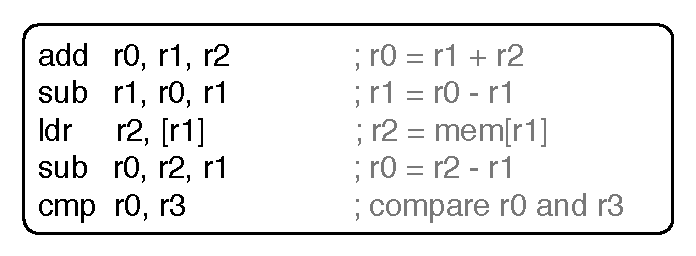
\includegraphics[scale=.65]{figs/sample_data_dependent_code}
  \end{center}
  \vspace{-3mm}
  \caption{Sample code with data dependencies}
  \label{fig:sample_data_dependent_code}
\end{wrapfigure}

Data hazards occur when the data needed by an instruction is not yet available.
Pipelines begin the execution of instructions before preceding ones are finished, so consecutive instructions that are data-dependent could simultaneously be executing in the pipeline.
For example, the code in figure~\ref{fig:sample_data_dependent_code} shows assembly instructions from the ARM instruction set architecture (ISA) that each depend on the result of its previous instruction.
Figure~\ref{fig:data_depend_execution_non_interleaved} shows two ways data hazards are commonly handled in pipelines. 

\begin{figure}
\vspace{-20pt} 
\begin{center}
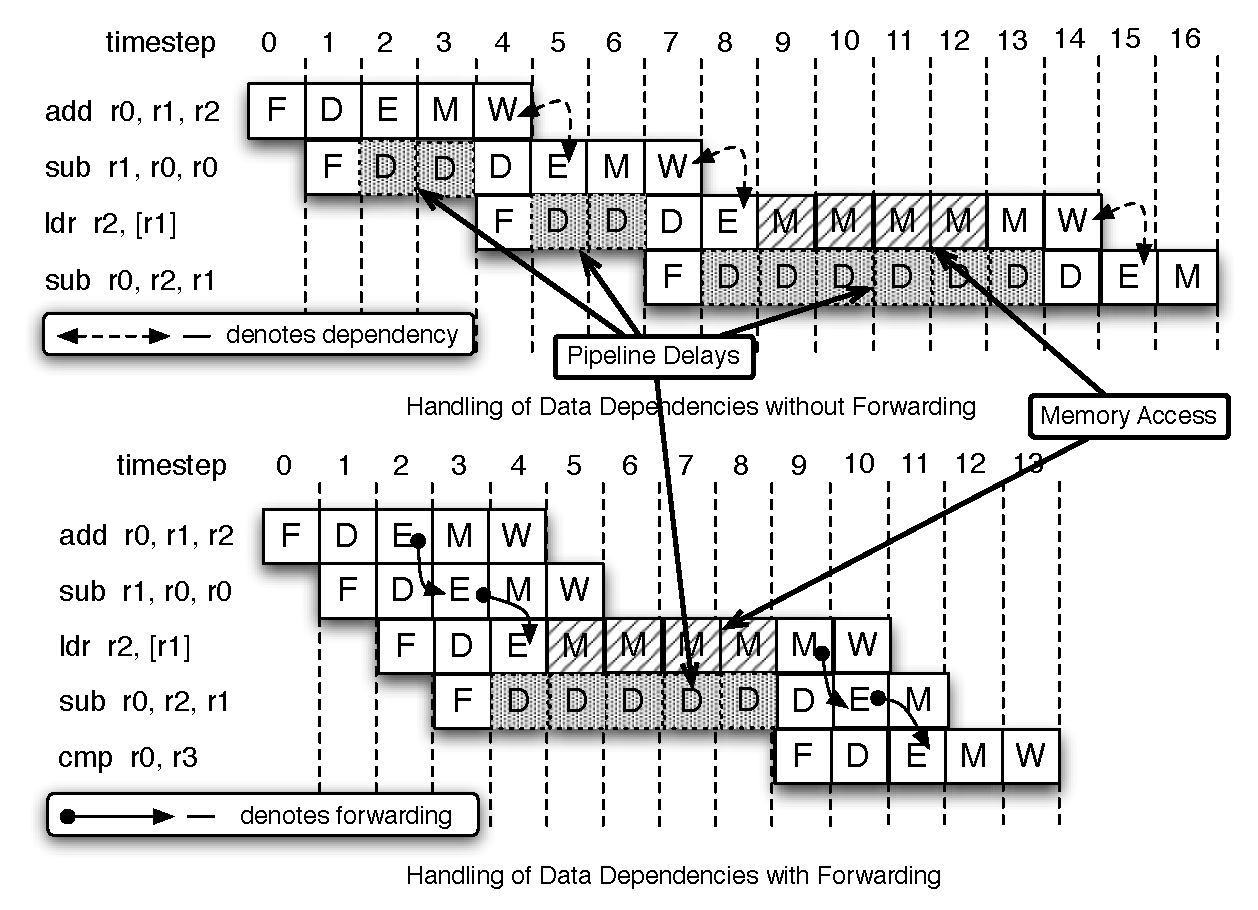
\includegraphics[scale=.6]{figs/data_depend_execution_non_interleaved}
\end{center}
\vspace{-3mm}
\caption{Handling of data dependencies in single threaded pipelines}
\label{fig:data_depend_execution_non_interleaved}
\end{figure}

In the figure, time progresses horizontally towards the right.
Each time step, or column, represents a processor cycle.
Each row represents an instruction that is fetched and executed within the pipeline.
Each block represents the instruction entering the different stages of the pipeline -- fetch (F), decode (D), execute (E), memory (M) and writeback (W).   
We assume a classic five stage RISC pipeline.

A simple but effective technique stalls the pipeline until the previous instruction completes.
This is shown in the top of figure~\ref{fig:data_depend_execution_non_interleaved}, as delays are inserted to wait for the results from previous instructions.
The dependencies between instructions are explicitly shown in the figure to make clear why the pipeline delays are necessary.
The performance penalty incurred in this case comes from the pipeline delays inserted.

\emph{Data forwarding} is commonly used to mitigate the need for inserting delays when data hazards occur.
Pipelines split up the execution of instructions into different execution stages. 
Thus, the results from an instruction could be ready, but waiting to be committed in the last stage of the pipeline.
Data forwarding utilizes this and introduces backwards data paths in the pipeline, so earlier pipeline stages can access the data from instructions in later stages that have not yet committed.
This greatly reduces the amount of delays inserted in the pipeline, as instructions can access the results of previous instructions before they commit.
The circuitry of data forwarding usually consists of the backwards data paths and multiplexers in the earlier pipeline stages to select the correct data to be used.    
The pipeline controller dynamically detects whether a data-dependency exists, and changes the selection bits of the multiplexers accordingly to select the correct operands.

The bottom of figure~\ref{fig:data_depend_execution_non_interleaved} shows the execution sequence of the previous example in a pipeline with data forwarding.
No pipeline delays are inserted for the first \emph{sub} and \emph{ldr} instruction because the data they depend on are forwarded with the forwarding paths.
However, delays are still inserted for the second \emph{sub} instruction after the \emph{ld} instruction.
For longer latency operations, such as memory accesses, the results are not yet available to be forwarded by the forwarding paths, so pipeline delays are still required. 
This illustrates the limitations of data forwarding.
They can address data hazards that result from pipelining, such as read-after-write register operations, but they cannot address data hazards that result from long latency operations, such as memory operations.
More involved techniques such as the out-of-order execution or superscalars are required to mitigate the effects of long latency operations.

The handling of data hazards in pipelines can cause instructions to exhibit dynamic execution times.  
For example, figure~\ref{fig:data_depend_execution_non_interleaved} shows the \emph{sub} instruction, in both top and bottom figures, exhibiting different execution times. 
To determine the execution time of instructions on pipelines that stall for data hazards, we need to determine when a stall is inserted, and how long the pipeline is stalled for.
Stalls are required when the current instruction uses the results of a previous instruction that is still in execution in the pipeline.
Thus, depending on the pipeline depth, a window of previous instructions needs to be checked to determine if any stalls are inserted.     
The length of the stall is determined by the execution time of the dependent instruction, because the pipeline will stall until that instruction completes.
Data forwarding does not remove the data hazards, but only reduces the number of stalls required to take care of the data hazards.  
Thus, to determine the execution time when data forwarding is used, timing analysis needs to determine when the data forwarding circuitry cannot not forward the data for data hazards.
This can similarly be done by observing the window of instructions not yet committed in the pipeline.  
The difference is, instead of all data dependencies, only data dependencies from long latency operations need to be detected.

Both techniques used for handling data hazards caused the execution time of instructions to depend on a window of previous instructions.
The deeper the pipeline, the larger the window of instructions execution time will depend on. 
Thus, static execution time analysis needs to model and account for this additional the window of instructions on pipelined architectures that use stalling or forwarding to handle the data hazards. 

\subsubsection{Control Hazards}
\begin{wrapfigure}{r}{0.5\textwidth}
  \vspace{-20pt}
  \begin{center}
    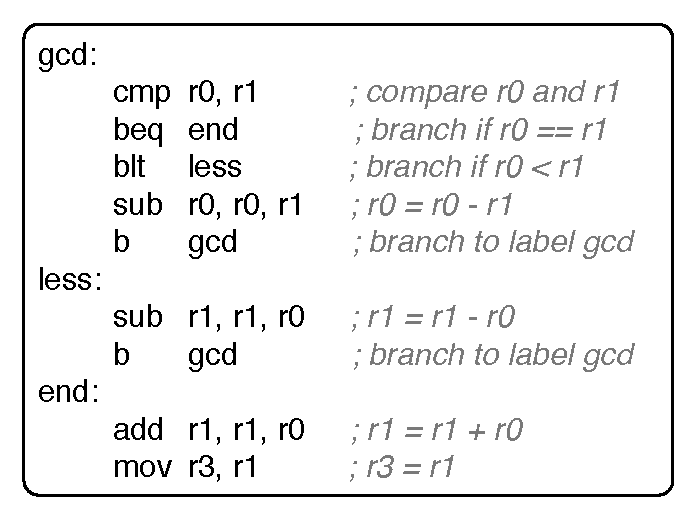
\includegraphics[scale=.65]{figs/sample_gcd_code}
  \end{center}
  \vspace{-3mm}
  \caption{GCD with conditional branches}
  \label{fig:sample_gcd_code}
\end{wrapfigure}

Branches are the most common cause of control-flow hazards (or control hazards) in the pipeline; the instruction after the branch, which should be fetched the next cycle, is unknown until after the branch instruction is completed.
Conditional branches further complicates matters, as whether or not the branch is taken depends on an additional condition that could also be unknown when the conditional branch is in execution. 
The code segment in figure~\ref{fig:sample_gcd_code} implements the \emph{Greatest Common Divisor} (GCD) algorithm using the conditional branch instructions \emph{beq} (branch equal) and \emph{blt} (branch less than) in the ARM ISA.  
Conditional branch instructions in ARM branch based on conditional bits that are stored in a processor state register.
Those conditional bits can be set based on the results of standard arithmetic instructions \todo{cite arm manual}.
The \emph{cmp} instruction is one such instruction that subtracts two registers and sets the conditional bits according to the results.
The GCD implementation shown in the code uses this mechanism to determine whether to continue or end the algorithm.
Figure~\ref{fig:branch_execution_non_interleaved_pipeline} shows the execution of the conditional branches from our example, and demonstrates two commonly used techniques to handling control hazards in pipelines. 
To show only the timing effects of handling control hazards, we assume an architecture with data forwarding that handles data hazards.
As there are no long latency instructions in our example, all stalls observed in the figure are caused by the handling of control hazards.  

\begin{figure}
\begin{center}
\noindent\makebox[\textwidth]{%
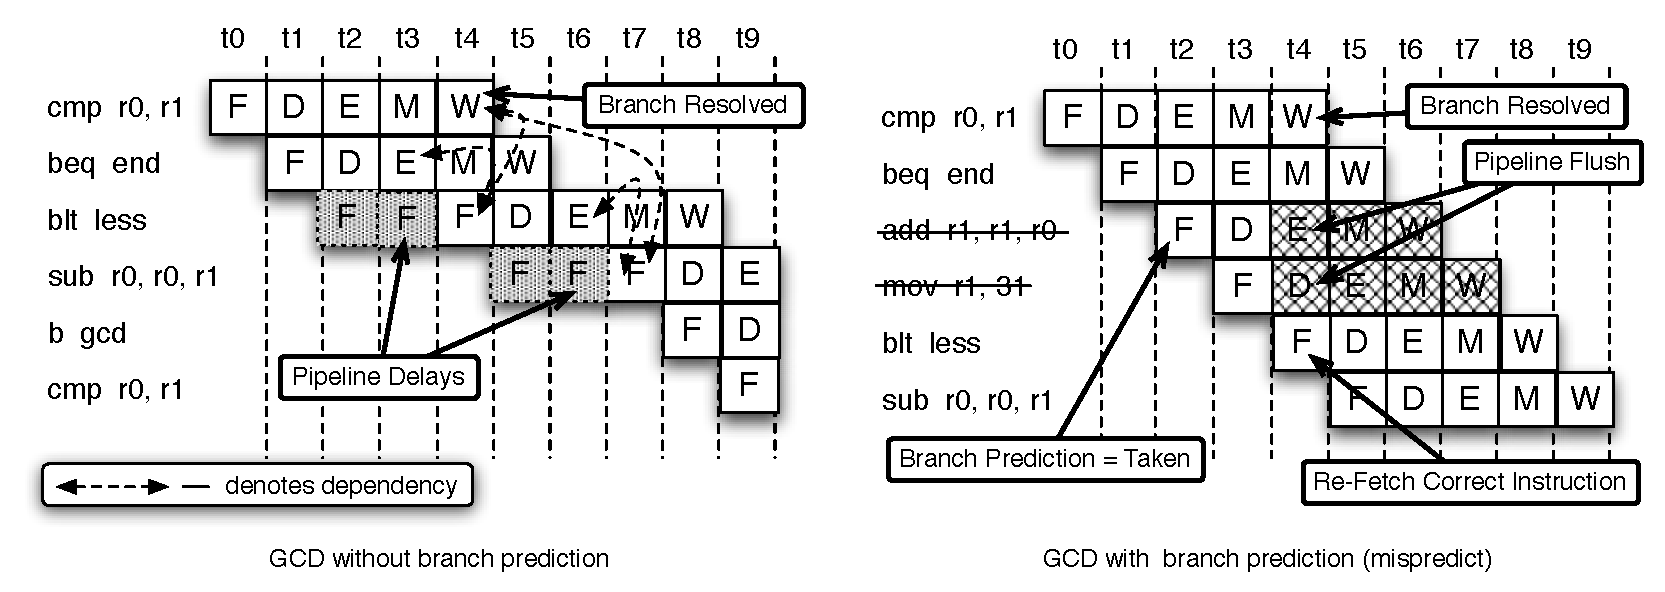
\includegraphics[scale=.58]{figs/branch_execution_non_interleaved_pipeline}}
\end{center}
\vspace{-3mm}
\caption{Handling of conditional branches in single threaded pipelines}
\label{fig:branch_execution_non_interleaved_pipeline}
\end{figure}

Similar to data hazards, control hazards can also be handled by stalling the pipeline until the branch instruction completes. 
This is shown on the left of figure~\ref{fig:branch_execution_non_interleaved_pipeline}. 
%The dependencies between instructions are explicitly shown to make clear why the pipeline delays are necessary.
Branch instructions typically calculate the target address in the execute stage, so two pipeline delays are inserted before the fetching of the \emph{blt} instruction, to wait for \emph{beq} to complete the target address calculation. 
The reasoning applies to the two pipeline delays inserted before the \emph{sub} instruction. 
The performance penalty (often referred to as the \emph{branch penalty}) incurred in this case is the two delays inserted after every branch instruction, to wait for the branch address calculation to complete.

To mitigate the branch penalty, some architectures enforce the compiler to insert one or more non-dependent instructions after each branch instruction.
These instruction slots are called branch delay slots, and are always executed before the pipeline branches to the target address. 
This way, instead of wasting cycles to wait for the target address calculation, the pipeline continues to execute useful instructions before it branches.
However, if the compiler cannot place useful instructions in the branch delay slot, \emph{nops} need to be inserted into those slots to ensure correct program execution.
Thus, branch delay slots are less effective for deeper pipelines because more delay slots need to be filled by the compiler to account for the branch penalty.
  
Instead of stalling, \emph{branch predictors} are commonly employed to predict the branch condition and target address so the pipeline can speculatively continue execution. 
Branch predictors internally maintain some form of state machine that is used to determine the prediction of each branch.  
The internal state is updated after each branch according to the results of the branch. 
Different prediction schemes have been proposed, and some can even accurately predict branches up to 93.5\%\todo{citation}.  
If the branch prediction is correct, no penalty is incurred for the branch because the correct instructions were speculatively executed.  
%With branch predictor, the pipeline fetches the next instruction based upon the results of the branch prediction, and continues to execute speculatively.
However, when the prediction is incorrect (often referred as a \emph{branch midpredict}), the speculatively executed instructions are flushed, and the correct instructions are re-fetched into the pipeline for execution.

The right of figure~\ref{fig:branch_execution_non_interleaved_pipeline} shows the execution of GCD in the case of a branch misprediction.
The \emph{beq} branch is predicted to be taken, so the \emph{add} and \emph{mov} instructions from label \emph{end} are directly fetched into execution. 
When \emph{beq} progresses past the execute stage, \emph{cmp} has forwarded its results used to determine the branch condition, and the branch target address has been calculated, so the branch is resolved.
At this point, the misprediction is detected, so the \emph{add} and \emph{mov} instruction are flushed out of the pipeline. 
The next instruction from the correct path, the \emph{blt} instruction, is immediately re-fetched, and execution continues.
The performance penalty of branch mispredictions is derived from the number of pipeline stages between instruction fetch and branch resolution.  
In our example, the misprediction penalty is 2, as branches are resolved after the execute stage.
This penalty only occurs on a branch mispredict, thus branch predictors with high success rates typically improve average performance of pipelines drastically, compared to architectures that simply stall for branches.
%However, for more complex architectures with caches or other hardware states, the effects of incorrectly fetched instructions on the state of the processor less well-known and studied. 

The two methods of handling control hazards exhibit vastly different effects on execution time.    
When stalls are used to handle control hazards, the execution time effects are static and predictable.   
The pipeline will simply \emph{always} insert pipeline delays after a branch instruction.
Thus, no extra complexity is added to the execution time analysis; the latency of branch instructions simply need to be adjusted to include the branch penalty.
On the other hand, if a branch predictor is employed, the execution time of each branch will vary depending on the result of the branch prediction.  
To determine the success of a branch prediction, both the prediction and the branch outcome, both of which can dynamically change in run-time, must be known.   
Program path analysis can attempt to analyze the actual outcome of branches statically from the program code. 
The predictions made from the branch predictor depend on the internal state stored in the hardware unit.
This internal state, updated by each branch instruction, must be explicitly modeled in order to estimate the prediction. 
If the predictor state is unknown, the miss penalty must conservatively be accounted for.
There has been work on explicitly modeling branch predictors for execution time analysis\todo{citation}, but the results are \todo{the results of branch predictor modeling for execution time analysis}.
To make matters worse, the speculative execution on the predicted program paths lead to further complications that need to be accounted for.
Other internal states exist in the architecture that could be affected by speculatively executing instructions.
For example, if caches were used, their internal state could be updated during speculative execution of a mispredicted path.
As architectures grow in complexity, the combined modeling of all hardware states in the architecture often lead to an infeasible explosion in state space for the analysis.    
This makes a tight static execution time analysis extremely difficult, if not impossible.

The difference in execution time effects between stalling and employing a branch predictor highlight an important trade-off for architecture designs.    
It is possible to improve average-case performance by making predictions, and speculatively executing based upon them.
However, this comes at the cost of predictability, and a potential prolonging of the worst-case performance.  
For real-time and safety critical systems, the challenge remains to improve worst-case performance while maintaining predictability.
How pipeline hazards are handled play an integral part of tackling this challenge.           
 
Although less often mentioned, the presence of interrupts and exceptions in the pipeline also create control hazards. 
Exceptions can occur during the execution of any instruction, and changes the control flow of the program to execute the exception handler.
For single threaded pipelines, this means that all instructions fetched and not committed in the pipeline are speculative, because when an exception occurs, all uncommitted instructions in the pipeline become invalid.
Pipelines often handle this by flushing all instructions and fetching the exception handler for execution.      
These effects are acknowledged, but often ignored in static analysis because it is simply impossible to model every possible exception, and its effect on the architecture states. 
 
\subsubsection{Structural Hazards}
\emph{Structural hazards} occur when a processor's hardware component is needed by two or more instructions at the same time. 
For example, a single memory unit accessed both in the fetch and memory stage results in a structural hazard. 
The design of the pipeline plays an integral part in eliminating structural hazards. 
For example, the classic RISC five stage pipeline only issues one instruction at a time, and uses separate instruction and data caches to avoid structural hazards.
Structural hazards are generally much more prevalent in architectures that issue multiple instructions at a time.
If structural hazards cannot be avoided, then the pipeline must stall to access the contended hardware component sequentially.
The execution time effects of structural hazards are specific to how contention is managed for each pipeline design.
Here we omit a general discussion of the timing effects, and later address them specifically for our proposed architecture. 

\subsection{Pipeline Multithreading}
Discussed above, \emph{data forwarding} and \emph{branch prediction} are simple techniques employed to handle pipeline hazards. 
Advanced architectures, such as \emph{superscalar} and \emph{VLIW} machines, employ more complex mechanisms to improve the average performance of the architecture.  
Both architectures issue multiple instructions every cycle, and superscalar machines dynamically execute instructions out-of-order if no dependency is detected.    
These architectures exploit \emph{instruction-level parallelism} to overlap the execution of instructions from a single thread whenever possible.         
On the contrary, \emph{multithreaded architectures} exploit \emph{thread-level parallelism} to overlap the execution of instructions from different hardware threads. 
Each hardware thread in a multithreaded architecture has its own physical copy of a processor state, such as the registers file and program counter etc.
When a pipeline hazard arises from the execution of a hardware thread, another hardware thread can be fetched for execution to avoid stalling the pipeline. 
This improves the instruction throughput of the architecture.

\begin{figure}[h]
\begin{center}
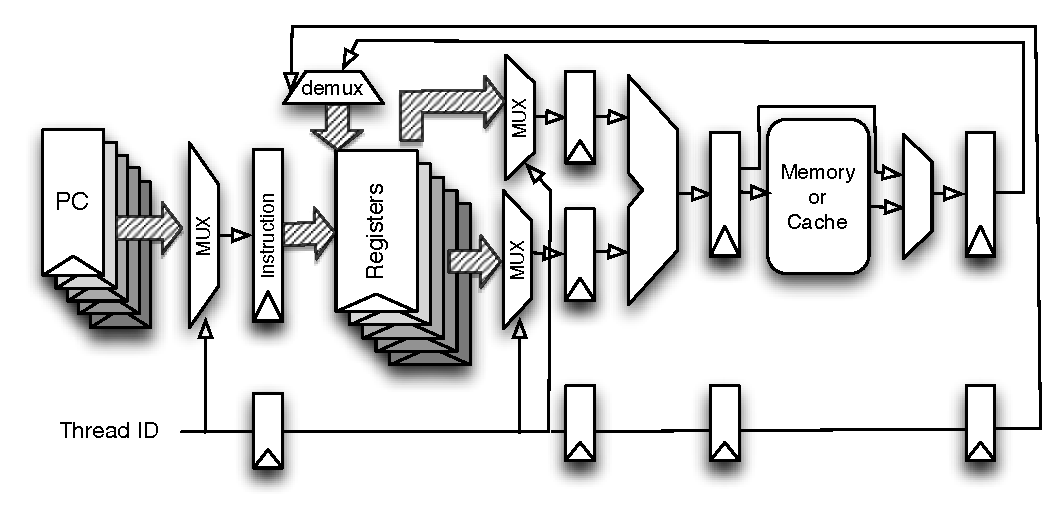
\includegraphics[scale=.8]{figs/multithreaded_pipeline_block}
\end{center}
\vspace{-10pt}
\caption{Simple Multithreaded Pipeline}
\label{fig:multi-thread pipeline simplified}
\end{figure}
Figure~\ref{fig:multi-thread pipeline simplified} shows the implementation of a simple multithreaded pipeline.
It contains 5 hardware threads, so it has 5 copies of the Program Counter (PC) and Register files.
The rest of the pipeline remains similar to a classic five stage RISC pipeline, with the addition of a few multiplexers used to select the thread states.
Thus, the extra copies of the processor state and multiplexers are most of the hardware additions needed to implement hardware multithreading.
When a hardware thread executes in the pipeline, its corresponding thread state is passed into the pipeline to be used.
In most of this thesis, the term \emph{threads} to refer to the explicit hardware threads that have hardware copies of the thread state.
This is not to be confused with the common notion of \emph{threads}, which describes software contexts managed by an operating system, with its states stored in memory.
It will be explicitly noted when we refer to the software notion of threads. 
%The selection of threads for execution is one of the most important factors to fully utilize thread-level parallelism.
%If a thread is stalled waiting for memory access but gets selected to execute in the pipeline, then that instruction slot is wasted and the processor isn't fully utilized.
Ungerer et al.~\cite{Ungerer:2003:survey_multithreading} surveyed different multithreaded architectures and categorized them based upon the \emph{thread scheduling} policy and the \emph{execution width} of the pipeline.

The \emph{thread scheduling} policy determines which threads are executing, and how often a context switch occurs.  
\emph{Coarse-grain} policies manage threads similar to the way operation systems manage software threads.
A thread gains access to the pipeline and continues to execute until a context switch is triggered.
Context switches occur less frequently via this policy, so less threads are required to fully utilize the processor.
Different coarse-grain policies trigger context switches with different events. 
Some policies trigger context switches on dynamic events, such as a cache miss or an interrupt; some policies trigger context switches on more static events, such as specialized instructions.
\emph{Fine-grain} policies switch context much more frequently -- some as frequent as every processor cycle.
The \emph{execution width} of the pipeline is to the number of instructions fetched each cycle.  
Multithreaded architectures with wider pipeline widths can fetch all instructions a single thread, or mix instructions from different threads.
The Sumultanous Multithreaded (SMT) architecture~\todo{cite} is an example where instructions are fetched from different threads each cycle.

Multithreaded architectures present several challenges for static execution time analysis.
As figure~\ref{fig:multi-thread pipeline simplified} illustrated, threads share the hardware components within the pipeline.
If a hardware component, such as a branch predictor, maintains internal state, that internal state can be modified by all threads in the pipeline.
As the internal states of the hardware components affect the execution time of the individual instructions, each thread can affect the execution time of all threads in the pipeline. 
If the threads' execution time are interdependent, their timing cannot be separately analyzed.
As a result, in order to precisely model the hardware states, the execution order of instructions from all threads need to be known.
The interleaving of threads depend heavily on the thread scheduling policy, execution width, and hazard handling logic employed in the pipeline.
The compounding effect of these can create an overwhelming combination of possible thread interleavings, making static timing analysis nearly impossible, even if only a conservative estimation is desired.   

Nonetheless, we contend that thread-level parallelism (TLP) \emph{can} be exploited to handle pipeline hazards predictably. 
Even the most sophisticated architectures that fully exploit instruction-level parallelism (ILP) cannot guarantee enough parallelism in a single instruction stream to remove all stalls caused by pipeline hazards. 
This is known as the \emph{ILP Wall}~\todo{cite}. 
Conventional multithreaded architectures use coarse-grain thread scheduling policies to dynamically exploit TLP when there is not enough ILP to be exploited.    
However, the compounding effects of the combined architectural features lead to unpredictable architectural timing behaviors.
Instead, a \emph{thread-interleaved pipeline} fully exploits TLP with a fine-grained thread scheduling policy.
We show that with several predictable architectural adjustments to the thread-interleaved pipeline, we can achieve a fully time-predictable pipeline 
with deterministic execution time behaviors.     

\subsection{A Predictable Thread-Interleaved Pipeline}
\label{section:pret_thread_pipeline}
Thread-interleaved pipelines use a fine-grain thread scheduling policy; every cycle a different hardware thread is fetched for execution.
A round robin scheduling policy is often employed to reduce the context switch overhead every cycle.     
The thread-interleaved pipeline is known for implementing the peripheral processors of the Cray Multi-Threaded Architecture (MTA) multiprocessors~\todo{cite}.
Each the ``peripheral processor'' is implemented as a hardware thread.     
Interacting with input/output peripherals often lead to idle processor cycles that waits for the peripherals' responses.
By interleaving several threads, thread-level parallelism is fully exploited, and the idle cycles can be used for simultaneous interaction with multiple input/output devices.       
Figure~\ref{fig:execution_thread_interleaved_pipeline} shows an example execution sequence from a 5 stage single width thread-interleaved pipeline with 5 threads.
\begin{figure}[h]
    \begin{center}
    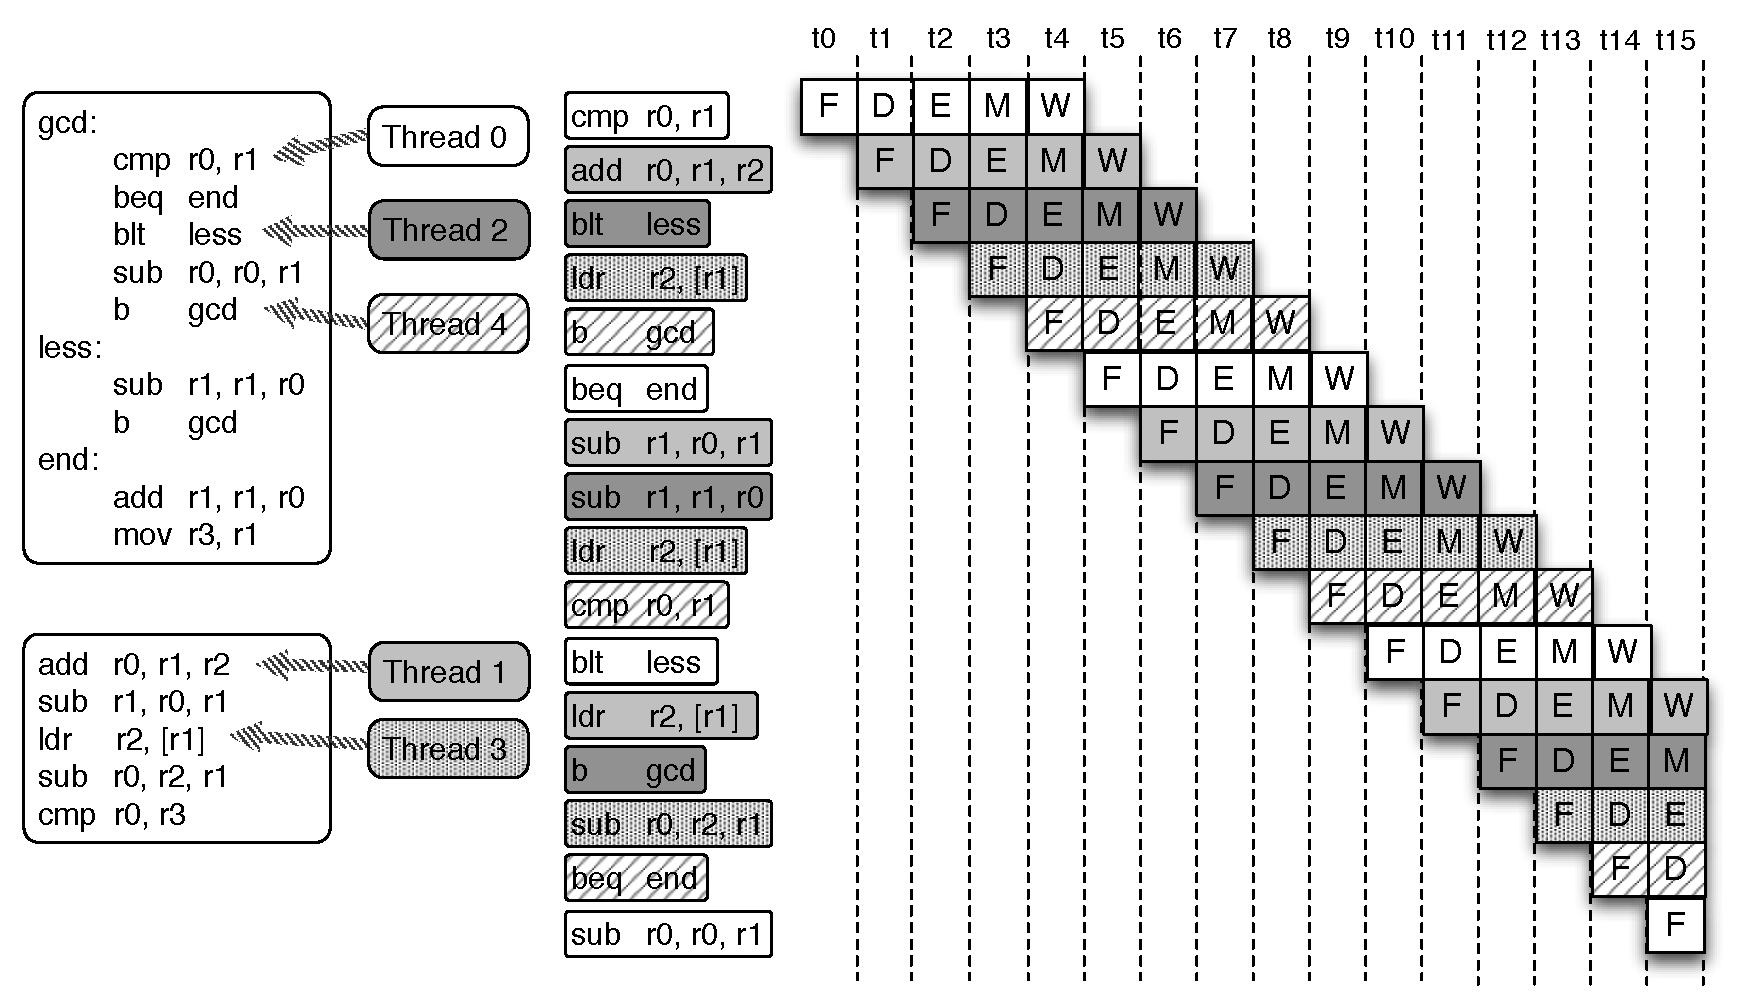
\includegraphics[scale=.55]{figs/thread-interleaved-execution}
  \end{center}
  \vspace{-10pt}
  \caption{Sample execution sequence of a thread-interleaved pipeline with 5 threads and 5 pipeline stages}
  \label{fig:execution_thread_interleaved_pipeline}
\end{figure}

The same code segments from figure~\ref{fig:sample_gcd_code} and figure~\ref{fig:sample_data_dependent_code} are used in this example. 
Threads 0, 2 and 4 execute GCD (figure~\ref{fig:sample_gcd_code}) and threads 1 and 3 execute the data dependent code segment (figure~\ref{fig:sample_data_dependent_code}).
The thick arrows on the left show the initial execution progresses of each thread at time 0.
We observe from the figure that each time step, an instruction from a different hardware thread is fetched in round robin order.
By time step 4, each pipeline stage is occupied by a different hardware thread.
The fine-grained thread interleaving and round robin scheduling combine to form this important property for thread-interleaved pipelines, which provides the basis for a timing predictable pipeline design.

The interleaving of threads by itself does not guarantee timing predictability for the pipeline.  
Shared hardware components or a selective thread execution policy can easily allow the execution time of threads to be affected by each other.    
As previously discussed, a combined timing analysis of all threads in the pipeline is extremely difficult, if not impossible.
In order for multithreaded architectures to achieve predictable performance, threads must be temporally isolated from one another. 
Temporal isolation removes cross-thread timing dependencies to allows timing analysis of threads independently.
This enables a simple and more precise execution time analysis.  
We refine several features on the thread-interleaved pipeline to temporally isolate the threads and predictably handle pipeline hazards.
This establishes a time-predictable thread-interleaved pipeline.

\subsubsection{Control Hazards}
By interleaving enough threads, control hazards can be completely removed from the pipeline.
This effect can be observed and explained from the execution sequence shown in figure~\ref{fig:execution_thread_interleaved_pipeline}.
At time 2, a \emph{blt} instruction from thread 2 is fetched into the pipeline.
On a single-threaded pipeline, stalls or branch prediction would be required to fetch the instruction at the next time step.
In this example, the next instruction fetched belongs to thread 3, and does not depend on the branch results of the \emph{blt} instruction.
No control hazard occurs from the branch, so no stall or branch prediction is needed to fetch the instruction.
The instruction fetch that depends on the branch result occurs at time 7.
Again, there is no control hazard since the branch is resolved by this point, so the instruction from the correct program path is fetched.    
Because control hazards from branches are eliminated, branch predictors are not needed in our pipeline design. 
Removing the branch predictor contributes to the temporal isolation of threads, as the shared internal state of the  branch predictor can create execution time dependencies between threads.  

The interleaving of threads also eliminate control hazards in the presence of exceptions.
If the pipeline detects an exception for the \emph{blt} instruction in the writeback stage (time 6), the control flow for thread 2 is changed to handle the exception.  
Because no other instruction in the pipeline belongs to thread 2 at time 6, no instruction needs to be flushed.  
This reveals an important property our timing predictable pipeline, that \emph{no instruction is speculatively executed}.
The next instruction fetch from thread 2 does not occur until time 7.
At that point, any control flow change, including one caused by an exception, is already known.
Therefore, the correct program path is always executed.

The minimum number of threads required to eliminate control hazards depend on the number of the pipeline stages.
Conservatively, employing the same number of threads as pipeline stages will always remove control hazards.
Intuitively, this is because at any point in time, each stage of the pipeline with be executing an instruction from a different hardware thread. 
Thus, no explicit dependency exists between instructions in the pipeline. 
However, Lee and Messerschmitt~\cite{lee1987pip} show that it is possible to use one less thread than the number of pipeline stages.
From here on, when we refer to the thread-interleaved pipeline, we assume enough threads to remove explicit dependencies between instructions in the pipeline.

\subsubsection{Data Hazards}
Because no explicit dependencies exist between instructions in the pipeline, data hazards that stem from the pipeline of instructions are removed. 
However, long latency operations can still cause data hazards in a thread-interleaved pipeline. 
This happens when a long latency operation is not completed before the next instruction fetch from the thread.
Although thread-interleaved pipelines can continue to fill the pipeline with other threads, data hazards are not completely eliminated.   
If all threads simultaneously execute a long latency operation, then no thread will be available to fill the pipeline. 

To maximizes pipeline utilization and instruction throughput, thread-interleaved pipelines can mark threads inactive when a long latency operation occurs.   
However, this dynamic behavior leads to non-trivial timing effects for the pipeline 
First, as stated earlier, a minimum number of threads is required to remove control hazards and the explicit dependencies between instructions in the pipeline. 
By allowing threads to be inactive, it is possible for the number of active threads to fall below this minimum. 
This can be circumvented by inserting pipeline stalls when the number active threads falls below the minimum.
This is illustrated in figure~\ref{fig:three_thread_pipeline}.
\begin{figure}[h]
  \vspace{-10pt}
  \begin{center}
    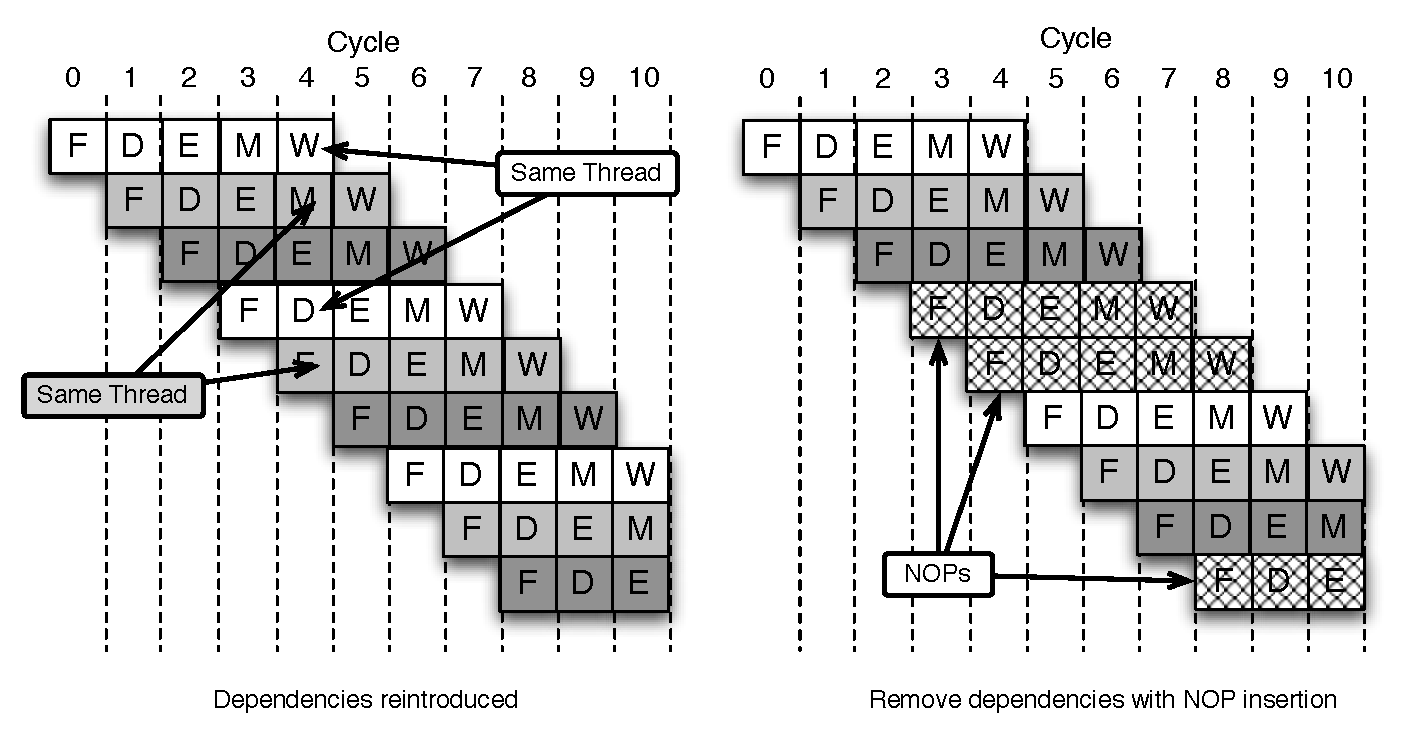
\includegraphics[scale=.6]{figs/three_thread_pipeline}
  \end{center}
  \vspace{-10pt}
  \caption{Execution of 5 threads thread-interleaved pipeline when 2 threads are inactive}
  \label{fig:three_thread_pipeline}
\end{figure}
This example shows the interleaving of 3 out of 5 threads in a 5 stage pipeline. 
We assume that 2 threads are inactive waiting for memory accesses.    
On the left we see that explicit dependency for instructions in the pipeline are reintroduced.
Only by inserting pipeline stalls to meet the minimum required thread count (shown on the right), can we assure that these dependencies are removed.   
The amount of stalling can be reduced if more threads are interleaved in the pipeline, since there is a larger pool of threads to select from. 
However, it is not possible to guarantee that stalls are never needed. 

More importantly, the dynamic activation and deactivation of threads breaks temporal isolation between the threads.   
When a thread is deactivated, other threads are fetched more frequently into the pipeline.
Thus, the execution frequency of threads would depend on number of active threads.
In order to maintain temporal isolation between the threads, our timing predictable thread-interleaved pipeline does not deactivate threads dynamically when long latency operations occur.

Instead, the thread scheduling policy of 

Although this slightly reduces the utilization of the thread-interleaved pipeline, but threads are decoupled and timing analysis can be done individually for each thread without interference from other threads.
At the same time, we still preserve most of the benefits of latency hiding, as other threads are still executing during the long latency operation.

%The next instruction from thread 3 that is fetched into the pipeline is again the same \emph{ld} instruction.  
%As memory completes its execution during the execution of instructions from other threads, we replay the same instruction to pick up the results from memory and write it into registers to complete the execution of the \emph{ld} instruction. 
%It is possible to directly write the results back into the register file when the memory operation completes, without cycling the same instruction to pick up the results.
%This would require hardware additions to support and manage multiple write-back paths in the pipeline, and a multi write ported register file, so contention can be avoided with the existing executing threads.
%In our design we simply replay the instruction for write-backs to simplify design and piggy back on the existing write-back datapath.

Because no explicit dependencies exist between instructions in the pipeline, data hazards that stem from the pipeline of instructions are removed. 
Thus, the forwarding logic normally used to handle data hazards are not needed in thread interleaved pipelines. 
Data forwarding logic contain no internal state, so threads can remain temporally isolated even if they are present.   
However, the pipeline design is greatly simplified in the absence of forwarding logic and branch predictors.   
This enables thread-interleaved pipelines to be clocked at faster clock speeds, because less logic exists between the pipeline stages.
  
\subsubsection{Structural Hazards}
Shared hardware units within multithreaded architectures could also easily break temporal isolation amongst the threads. 
Two main issues arise when a hardware unit is shared between the threads. 
The first issue arises when shared hardware units share the same state between all threads. 
If the state of hardware unit is shared and can be modified by any thread, then it is nearly impossible to get a consistent view of the hardware state from a single thread during timing analysis.
Shared branch predictors and caches are prime examples of how a shared hardware state can cause timing inference between threads.
If a multithreaded architecture shares a branch predictor for all threads, then the branch table entries can be overwritten by branches from any thread.
This means that each thread's branches can cause a branch mispredict for any other thread. 
Caches are especially troublesome when shared between threads in a multithreaded architecture. 
Not only does it make the execution time analysis substantially more difficult, it also decreases overall performance for each thread due to cache thrashing, an event where threads continuously evict each other threads cache lines in the cache\todo{citation}.
To achieve temporal isolation between the threads, the hardware units in the architecture must not share state between the threads. 
Each thread must have its own consistent view of the hardware unit states, without the interference from other threads.
For example, each thread in our thread-interleaved pipeline contains its own private copy of the registers and thread states.    
We already showed why thread-interleaved pipelines do not need branch predictors because they remove control-hazards, and we will discuss a timing predictable memory hierarchy that uses scratchpads instead of caches in section~\ref{section:memory_system}.
The sharing of hardware state between threads also increases security risks in multithreaded architectures. 
Side-channel attacks on encryption algorithms\todo{cite} take advantage of the shared hardware states to disrupt and probe the execution time of threads running the encryption algorithm to crack the encryption key.
We will discuss this in detail in section~\ref{sec:app_side_channel_attack} and show how a predictable architecture can prevent timing side-channel attacks for encryption algorithms.   

The second issue that arises is that shared hardware units create structural hazards -- hazards that occur when a hardware unit needs to be used by two or more instructions at the same time.
Structural hazards typically occur in thread-interleaved pipelines when the shared units take longer than one cycle to access. 
The ALU, for example, is shared between the threads.
But because it takes only one cycle to access, there is no contention even when instructions continuously access the ALU in subsequent cycles.
On the other hand, a floating point hardware unit typically takes several cycles to complete its computation.
If two or more threads issue a floating point instruction in subsequent cycles, then contention arises, and the the second request must be queued up until the first request completes its floating point computation.   
This creates timing interference between the threads, because the execution time of a floating point instruction from a particular thread now depends on if other threads are also issuing floating point instructions simultaneously. 
If the hardware unit can be pipelined to accept inputs every processor cycle, then we can remove the the contention caused by the hardware unit, since accesses no longer need to be queued up.
The shared memory system in a thread-interleaved pipeline also creates structural-hazards in the pipeline.
In section~\ref{section:memory_system} we will discuss and present our memory hierarchy along with a redesigned DRAM memory controller that supports pipelined memory accesses.
%The assumption here is still that we have a single issue pipeline architecture.   
If pipelining cannot be achieved, then any timing analysis of that instruction must include a conservative estimation that accounts for thread access interference and contention management.
Several trade-offs need to be considered when deciding how to manage the thread contention to the hardware unit.

A time division multiplex access (TDMA) schedule to the hardware unit can be enforced to decouple the access time of threads remove timing interference.
A TDMA access scheme certainly creates an non-substantial overhead compared to conventional queuing schemes, especially if access to the hardware unit is rare and sparse.
However, in a TDMA scheme, each threads wait time to access the shared resource depends on the time offset in regards to the TDMA schedule, and is decoupled from the accesses of other threads.
Because of that, it is possible obtain a tighter worst case execution time analysis per thread.
For a TDMA scheme, the worst case access time occurs when an access just missed its time slot and must wait a full cycle before accessing the hardware unit.
For a conventional queuing scheme where each requester can only have one outstanding request, the worst case happens when every other requester has a request in queue, and the first request is just beginning to be serviced.   
At first, it may seem that the worst case execution time of a TDMA scheme may seem similar to the basic queuing scheme.
For timing analysis at an unknown state of the program, no assumption can be made on the TDMA schedule, thus the worst case time must be used for conservative estimations. 
However, because the TDMA access schedule is static, and access time is decoupled from other threads, there is potential to obtain tighter timing analysis for accesses by inferring access slot hits and misses for future accesses. 
For example, based upon the execution time offsets of a sequence of accesses to the shared resource, we may be able to conclude that at least one access will hit its TDMA access slot and get access right away.
We can also possibly derive more accurate wait times for the accesses that do not hit its access slots based upon the elapsed time between accesses.
An in depth study of WCET analysis of TDMA access schedules is beyond the scope of the thesis.
But these are possibilities now because there is no timing interference between the threads. 
A queue based mechanism would not be able to achieve better execution time analysis without taking into account the execution context of all other threads in the pipeline.

\bigskip

\todo{Compare execution sequences of previous figures of threads. Highlight the simpler timing analysis}

\todo{highlight that the observable latency of long latency instructions are predictably reduced}
For operations that have long latencies, such as memory operations or floating point operations, thread-interleaved pipelines hides the latency with its execution of other threads. 
Thread 3 in figure~\ref{fig:execution_thread_interleaved_pipeline} shows the execution of a \emph{ld} instruction that takes the same 5 cycles as shown in figure~\ref{fig:data_depend_execution_non_interleaved}.
We again assume that this \emph{ld} instruction accesses data from the main memory. 
While the \emph{ld} instruction is waiting for memory access to complete, the thread-interleaved pipeline executes instructions from other threads.

It is important to understand that we are not proclaiming that all dynamic behavior in systems are harmful. 
But only by achieving predictability in the hardware architecture can we begin to reason about more dynamic behavior in software.
For example, we discussed that dynamically scheduling threads in hardware causes timing interference. 
However, it is not the switching of threads that is unpredictable, but how the thread switching is triggered that makes it predictable.   
For example, the Giotto\todo{cite} programming model specifies a periodic software execution model that can contain multiple program states. 
If such a programming model was implemented on a thread-interleaved pipeline, different program states might map different tasks to threads or have different number of threads executing within the pipeline.
But by explicitly controller the thread switches in software, the execution time variances introduced is transparent at the software level, allowing potential for timing analysis.

%TODO: Talk about the trade-offs of threaded interleaved pipelines to summarize 
In this section we introduced a predictable thread-interleaved pipeline design that provides temporal isolation for all threads in the architecture.
The thread-interleaved pipeline favors throughput over single thread latency, as multiple threads are executed on the pipeline in a round robin fashion.  
We will present in detail our implementation of this thread-interleaved pipeline in chapter~\ref{chapter:ptarm}, and show how the design decisions discussed in this chapter are applied.

\section{Memory System}
\label{section:memory_system}
While pipelines designs continue to improve, memory technology has been struggling to keep up with the increase in clock speed and performance.
Even though memory bandwidth can be improved with more bank parallelization, the memory latency remains the bottleneck to improved memory performance.
Common memory technologies used in embedded systems contain a significant tradeoff between access latency and capacity. 
Static Random-Access Memories (SRAM) provide a shorter latency that allows single cycle memory access from the pipeline.
However, the hardware cost to implement each memory cell prevents SRAM blocks from being implemented with high capacity.
On the other hand, Dynamic Random-Access Memories (DRAM) use a more compact memory cell design that can easily be combined into larger capacity memory blocks.
But the memory cell of DRAMs must be constantly refreshed due to charge leakage, and the large capacity memory blocks often prohibit faster access latencies.
%TODO: talk about about embedded systems seldom need disk?
To bridge the latency gap between the pipeline and memory, smaller memories are placed in between the pipeline and larger memories to act as a buffer, forming a memory hierarchy.
The smaller memories give faster access latencies at the cost of lower capacity, while larger memories make up for that with larger capacity but slower access latencies. 
The goal is to speed up program performance by placing commonly accessed values closer to the pipeline and placing less accessed values farther away.

\subsection{Memory Hierarchy}
\subsubsection{Caches}
\begin{wrapfigure}{r}{0.5\textwidth}
  \vspace{-20pt}
  \begin{center}
    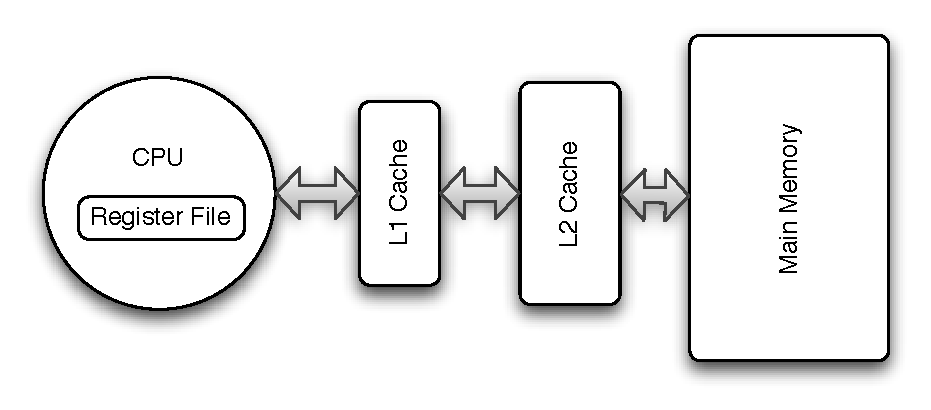
\includegraphics[scale=.5]{figs/conventional_mem_hierarchy}
  \end{center}
  \vspace{-20pt}
  \caption{Memory Hierarchy w/ Caches}
  \label{fig:conventional_mem_hierarchy}
  \vspace{-10pt}
\end{wrapfigure}   
A \emph{CPU Cache} (or cache) is commonly used in the memory hierarchy to manage the smaller fast access memory made of SRAMs.
The cache manages the contents of the fast access memory in hardware by leveraging the spatial and temporal locality of data accesses. 
The main benefits of the cache is that it abstracts away the memory hierarchy from the programmer.
When a cache is used, all memory accesses are routed through the cache. 
If the data from the memory access is in the cache, then a cache hit occurs, and the data is returned right away.
However, if data is not in the cache, then a cache miss occurs, and the cache controller fetches the data from the larger memory and adjusts the memory contents in the cache. 
The replacement policy of the cache is used to determine which cache line, the unit of memory replacement on caches, to replace. 
A variety of cache replacement policies have been researched and used to optimize for different memory access patterns of applications. 
In fact, modern memory hierarchies often contain multiple layers of hierarchy to balance the tradeoff between speed and capacity.
A commonly used memory hierarchy is shown in figure~\ref{fig:conventional_mem_hierarchy}.
If the data value is not found in the L1 cache, then it is searched for in the L2 cache. 
If the L2 cache also misses, then the data is retrieved from main memory, and sent back to the CPU while the L1 and L2 cache update its contents.
Different replacement policies can be used at different levels of the memory hierarchy to optimize the hit rate or miss latency of the memory access.

When caches are used, the program is oblivious to the different levels of memory hierarchy because they are abstracted away from the program; the cache gives its best-effort to optimize memory access latencies.
Whether or not an access hits the cache or goes all the way out to main memory is hidden from the program.
Thus, the programmer does not need to put in any effort, and can get a reasonable amount of performance. 
Furthermore, when programs are ported to another architecture with a different cache configuration, no change in the program is required to still obtain a reasonable amount of performance from the hardware.   
For general purpose applications, this gives the ability to improve design time and decrease design effort, which explains the cache's popularity. 

However, the cache makes no guarantees on actual memory access latencies and program performance. 
The execution time of programs could highly vary depending on a number different factors -- cold starts, previous execution contexts, interrupt routines, and even branch mispredictions that cause unnecessary cache line replacements.  
Thus, when execution time is important, the variability and uncontrollability of caches may outweigh the benefits they provide. 

The cache's internal states include the controller state and memory contents. 
As the programmer cannot explicitly control the state of the cache, it is extremely difficult to analyze execution time on systems with caches.
At an arbitrary point of execution, if the state of the cache is unknown, a conservative worst-case execution time analysis needs to assume the worst case, as if the memory access went directly to main memory.
In order to acquire tighter execution time analysis, the cache must be modeled with program execution to predict the cache state.
The ease of such modeling depends on the replacement policy used in the cache.

For example, the \emph{Least Recent Used} (LRU) replacement policy replaces the least recently used cache line whenever an eviction occurs. 
Within a basic block, a code segment without a control flow change, the contents of a cache with $N$ cache lines can be fully known after $N$ different memory accesses~\cite{Heckmann2003processor}.  
The $N$ different memory accesses will evict all cache lines in the cache prior to the basic block, and fill them with the memory contents of the $N$ accesses. 
In this case, the analysis assumes $N$ initial cache misses before the cache state is known.
However, the cache state is destroyed when analysis hits a control flow merge with another path.
Thus, the usefulness of this analysis depends on $N$ and how long basic blocks are in programs.  
In practice, the complexity of modern programs and memory architectures often introduce a high variability in program execution time, rendering analysis imprecise. 

Even outside of the context of real-time applications, caches can present unintended side effects.
For applications that require extreme high speed, the best-effort memory management that caches offer simply is not good enough.
Programs often need to be tuned and tailored to specific cache architectures and parameters to achieve the desired performance. 
In order to tune algorithm performance, algorithm designers are required to understand the abstracted away memory architecture and enforce data access patterns that conform to the cache size and replacement policy.   
For example, instead of operating on entire rows or columns of an array, algorithms are rewritten to operate on a subset of the data at a time, or blocks, so the faster memory in the hierarchy can be reused.
This technique is called \emph{Blocking}~\cite{Lam91thecache}, and is very well-known and commonly used.   
%\todo{talk about LAPACK? Libraries that tune programs to caching}.
%In this case, we see that the hidden memory hierarchy actually could degrade program performance.    

Multithreaded threaded architectures with shared caches among the hardware threads can suffer from \emph{cache thrashing}, an effect where different threads' memory accesses evict the cached lines of others.
With multiple hardware threads, it is extremely difficult for threads have any knowledge on the state of the cache, because it is simultaneously being modified by other threads in the system. 
As a result, the hardware threads have no control over which level in the memory hierarchy they are accessing, and the performance highly varies depending on what is running on other hardware threads. 

For multicore architectures, caches create a data coherency problem when data needs to be consistent between the multiple cores.
When the multiple cores are sharing memory, each core's private cache may cache the same memory address. 
If one core writes to a memory location that is cached in its private cache, then the other core's cache would contain stale data. 
Various methods such as bus snooping or implementing a directory protocol~\cite{Stenstrom:1990:SCC:79809.79810} have been proposed to keep the data consistent in all caches. 
Implementing a scalable and efficient cache coherence scheme is still a hot topic of research today.

\subsubsection{Scratchpads}
We cannot argue against the need for a memory hierarchy, as there is an undeniable gap between processor and DRAM latency.
However, instead of abstracting away the memory hierarchy, we propose to \emph{expose} the memory layout to the software.  

\emph{Scratchpads} were initially proposed for their power saving benefits over caches~\cite{Banakar2002}.
Scratchpads can be found in the Cell processor~\cite{cellproc}, which is used in Sony PlayStation 3 consoles, and NVIDIA's 8800 GPU, which provides 16KB of SPM per thread-bundle~\cite{8800gpu}.
Scratchpads use the same memory technology (SRAMs) as caches, but do not implement the hardware controller to manage their memory contents.
%Without the hardware controller, scratchpads do not manage its memory contents in hardware.
Instead, scratchpads occupy a distinct address space in memory when they are used as fast access memory.
Memory accesses that access the specific scratchpad address space will go to the scratchpad, and other accesses will go to main memory. 
Because in hardware scratchpads do not need to check whether the data is on the scratchpad or not, they have a reduced access latency, area and power consumption compared to caches~\cite{Banakar2002}. 

\begin{wrapfigure}{r}{0.45\textwidth}
  \vspace{-20pt}
  \begin{center}
    \includegraphics[scale=.5]{figs/pret_mem_hierarchy}
  \end{center}
  \vspace{-10pt}
  \caption{Memory Hierarchy w/ Scratchpads}
  \label{fig:pret_mem_hierarchy}
\end{wrapfigure}   

Unlike caches, which overlay their address space with main memory to hide the hierarchy, scratchpads explicitly \emph{expose} the memory hierarchy, as figure~\ref{fig:pret_mem_hierarchy} illustrates.  
The exposed memory hierarchy gives software full control over the management of memory contents in the hierarchy.
Data allocated on the scratchpad will have single cycle access latencies, while other data will take the full DRAM access latency. 
The memory access latency for each request now depends only on the access address, and not that state of another hardware controller. 
This drastically improves the predictability of memory access times, and removes the variability of execution time introduced with caches.
However, this places the burden of memory management on the programmer or compiler toolchains.  
The Cell processor~\cite{cellproc} is often criticized for being difficult to program, and one of the main reason is its use of scratchpads. 
Programmers have become accustomed to a uniform memory space, making it difficult to adjust to the non uniform memory space that must be explicitly managed.

Embedded system designs inherently need to deal with limited resources and other design constraints, such as limited memory or hard timing deadlines.    
Thus, the design of such systems often requires analysis of memory usage and latency to ensure that the constraints are met.
These analysis results can be used to generate automatic allocation schemes for scratchpads, lessening the burden on programmers.
Two allocation schemes are commonly employed to manage the contents of scratchpads in software.
\emph{Static allocation schemes} allocate data on the scratchpad during compile time, and the contents allocated on the scratchpad do not change throughout program execution. 
Static scratchpad allocation schemes~\cite{Suhendra2005WCETSPM, Patel2008PRETSPM} often use heuristics or a compiler-based static analysis of the program to find the most commonly executed instructions or data structures.
These are allocated statically on the scratchpad to improve program performance. 
\emph{Dynamic allocation schemes} modify the data on the scratchpad during run time in software through DMA mechanisms.
The allocation could either be automatically generated and inserted by the compiler, or explicitly specified by the user programmatically.
Higher level models of computation, such as Synchronous Dataflow (SDF)~\cite{lee_sdf} or Giotto~\cite{henzinger_giotto}, expose more structure and semantics of the model for better analysis, which can be used to optimize scratchpad allocation dynamically.
Bandyopadhyay~\cite{Bandyopadhyay06_AutomatedMemoryAllocationOfActorCodeDataBufferInHeterochronous} presents an automated memory allocation of scratchpads for the execution of Heterochronous Dataflow models.
The Heterochronous Dataflow (HDF) model is an extension to the Synchronous Dataflow (SDF) model with finite state machines (FCM). 
The HDF models contain different program states.
Each state executes a SDF model that contains actors communicating with each other. 
Bandyopadhyay analyzes the actor code and the data that is communicated in each HDF state, and derives an optimized scratchpad allocation for each state. 
The scratchpad allocation code is automatically inserted into the code to dynamically change the scratchpad contents during state transitions, so the memory allocation is optimized for the execution of each HDF state. 
This allocation not only shows roughly a 17\% performance improvement compared to executions using LRU caches, but also a more predictable program performance.

The underlying memory technology that is used to make both scratchpads and caches is not inherently unpredictable, as SRAMs provide constant low-latency access time. 
%However, caches manage the contents of the SRAM in hardware. 
However, by using caches in the memory hierarchy, the hierarchy is hidden from the programmer, and the hardware managed memory contents create highly variable execution times with unpredictable access latencies. 
Scratchpads on the other hand expose the memory hierarchy to the programmer, allowing for more predictable and repeatable memory access performances.
Although the allocation of scratchpads requires more programming effort, it also provides opportunity for high efficiency, as it can be tailored to specific applications.   
Thus, in our time-predictable architecture, scratchpads are employed as our fast-access memory. 

\subsection{DRAM Memory Controller}
Because of its high capacity, DRAMs are often employed in modern embedded systems to cope with the increasing code and data sizes.  
However, bank conflicts and refreshes within the DRAM can cause memory accesses to stall, further increasing the memory latency. 
Modern memory controllers are designed to optimize average-case performance by queueing and reordering memory requests to improve the throughput of memory requests. 
This results in unpredictable and varying access times along with an increased worst-case access time for each memory request.
In this section we will present a DRAM memory controller that privatizes DRAM banks with scheduled memory refreshes to provide improved worst-case latency and predictable access times.    
The contributions from this section are research done jointly with the several co-authors from Reineke et. al~\cite{ReinekeLiuPatelKimLee11_PRETDRAMControllerBankPrivatizationForPredictability}. 
We do not claim sole credit for this work, and the summary is included in this thesis only for completeness. 
We will first give some basic background on DRAM memories, then present the predictable DRAM controller designed.

\subsubsection{DRAM Basics}

\begin{figure}[h]
\begin{center}
\vspace{-8mm}
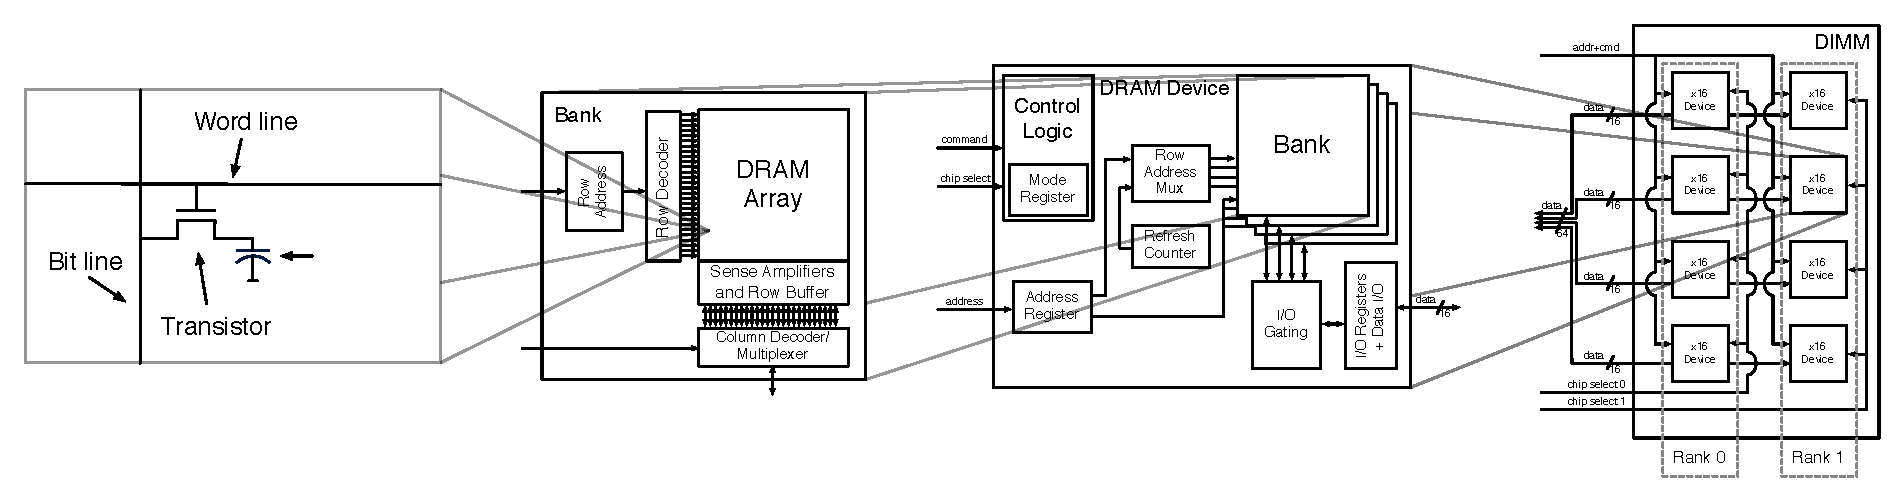
\includegraphics[width=\textwidth]{figs/dram-overview.pdf}
\vspace{-8mm}
\caption{A dual-ranked dual in-line memory module.}\label{fig:dram_basics}
\vspace{-5mm}
\end{center}
\end{figure} 

Figure~\ref{fig:dram_basics} shows the structure of a dual ranked in-line DDRII DRAM module.
Starting from the left, a basic \textbf{\emph{DRAM cell}} consists of a capacitor and a transistor. 
The capacitor charge determines the value of the bit, which can be accessed by triggering the transistor. 
Because the capacitor leaks charge, it must be refreshed periodically, typically every 64 ms or less~\cite{jedec}.

A \textbf{\emph{DRAM array}} is made of a two-dimensional array of DRAM cells.
Each access made to the DRAM array goes through two phases: a row access followed by one or more column accesses.   
During the row access, one of the rows in the DRAM array is moved into the row buffer.
To read the value in the row buffer, the capacitance of the DRAM cells is compared to the wires connecting them with the row buffer.
The wires need to be precharged close to the voltage threshold so the sense amplifiers can detect the bit value.
Columns can be read and written to quickly after the row is in the row buffer. 

The \textbf{\emph{DRAM device}} consists of banks formed of DRAM arrays. 
Modern DRAM devices have multiple banks, control logic, and I/O mechanisms to read from and write to the data bus, as shown in the center of figure \ref{fig:dram_basics}.
Banks can be accessed concurrently, but the data, command and address busses, which is what the memory controller uses to send commands to the DRAM device, are shared within the device. 
The following table\footnotemark\ lists the four most important commands and their function:
\footnotetext{This table is as shown in ~\cite{ReinekeLiuPatelKimLee11_PRETDRAMControllerBankPrivatizationForPredictability}}
%\begin{table}
\begin{center}
\begin{smalltabular}{p{13mm}p{6mm}p{10cm}}
Command 				& Abbr. & Description\\\hline
Precharge    			& PRE   & Stores back the contents of the row buffer into the DRAM array, and prepares the sense amplifiers for the next row access.\\
Row\hspace{13mm} access & RAS	& Moves a row from the DRAM array through the sense amplifiers into the row buffer.\\
Column access 			& CAS   & Overwrites a column in the row buffer or reads a column from the row buffer.\\
Refresh					& REF	& Refreshes several\footnotemark\ rows of the DRAM array. This uses the internal refresh counter to determine which rows to refresh.\\
\end{smalltabular}
%\caption{Overview of DDR2 Commands~\cite{ReinekeLiuPatelKimLee11_PRETDRAMControllerBankPrivatizationForPredictability}}
\label{tab:ddr2-commands}
\end{center}
%\end{table}
\footnotetext{The number of rows depends on the capacity of the device.}

To perform reads or writes, the controller first sends the PRE command to precharge the bank containing the data. 
Then, a RAS is issued to select the row, and one or more CAS commands can be used to access the columns within the row. 
Accessing columns from the same row does not require additional PRE and RAS commands, thus higher throughput can be achieved by performing column accesses in burst lengths of four to eight words.  
Column accesses can immediately be followed by a PRE command to decrease latency when accessing different rows. 
This is known as auto-precharge (or closed-page policy).
Refreshing of the cells can be done in two ways.
One common way is to issue a refresh command that refreshes all banks of the device simultaneously. 
The refresh latency depends on the capacity of the device, but the DRAM device manages a counter to step through all the rows.
The rows on the device could also be manually refreshed by performing row accesses to them.
Thus, the memory controller could perform row accesses on every row within the 64 ms refresh period.
This requires the memory controller to keep track of the refresh status of the device and issue more refresh commands, but each refresh takes less time because it is only a row access. 

\textbf{\emph{DRAM modules}} are made of several DRAM devices integrated together for higher bandwidth and capacity. 
A high-level view of the dual-ranked dual in-line memory module (DIMM) is shown in the right side of figure~\ref{fig:dram_basics}.
The DIMM has eight DRAM devices that are organized in two ranks.
The two ranks share the address, command inputs, and the 64-bit data bus.
The chip select is used to determine which ranks are addressed.
All devices within a rank are accessed simultaneously when the rank is addressed, and the results are combined to form the request response.  
% Due to the sharing of I/O mechanisms within a device, consecutive accesses to the same rank are more constrained than consecutive accesses to different ranks, which only share the command and address as well as the data bus.
% We later exploit this subtle difference by restricting consecutive accesses to different ranks to achieve more predictable access latencies.  
% We explain this in more detail in \ref{sec:pret_dram_controller}. 

Our controller makes use of a feature from the DDR2 standard known as posted-CAS.  
Unlike DDR or other previous versions of DRAMs, DDR2 can delay the execution of CAS commands (posted-CAS) for a user-defined latency, known as the additive latency ($AL$). 
Posted-CAS can be used to resolve command bus contention by sending the posted-CAS earlier than the corresponding CAS needs to be executed.

Table~\ref{table:ddr2-constraints} gives an overview of timing parameters for a DDR2-400 memory module.
These timing constraints come from the internal structure of DRAM modules and DRAM cells.
For example, $t_{RCD}, t_{RP}$, and $t_{RFC}$ are from the structure of DRAM banks that are accessed through sense amplifiers that need to be precharged.
$t_{CL}, t_{WR}, t_{WTR}$, and $t_{WL}$ result from the structure of DRAM banks and DRAM devices.
The four-bank activation window constraint $t_{FAW}$ constrains rapid activation of multiple banks that would result in too high of a current draw.
The memory controller must conform to these timing constraints when sending commands to the DDR2 module.  
%The additive latency, $t_{AL}$, can be set by the user and determines how many cycles after a posted-CAS a CAS is executed.
Here we only give a quick overview of DRAMs, we refer more interested readers to Jacob et al.~\cite{JaNgWa07} for more details.

\begin{table}[h]
\begin{center}
\begin{smalltabular}{l p{2.0cm} p{10cm}}
Parameter	& Value \footnotemark & Description \\\hline
$t_{RCD}$			& 3						& \textbf{Row-to-Column delay}: time from row activation to first read or write to a column within that row.\\
$t_{CL}$			& 3						& \textbf{Column latency}: time between a column access command and the start of data being returned.\\
$t_{WL}$			& $t_{CL}-1=2$			& \textbf{Write latency}: time after write command until first data is available on the bus.\\
$t_{WR}$			& 3						& \textbf{Write recovery time}: time between the end of a write data burst and the start of a precharge command.\\
%$t_{CCD}$			& $\burstlength/2$ 				& CAS to CAS command delay. Minimum time between two read commands or two write commands.\\
$t_{WTR}$ 			& 2 					& \textbf{Write to read time}: time between the end of a write data burst and the start of a column-read command.\\% Allows the sense amplifiers to restore the data in the DRAM array.\\
$t_{RP}$			& 3						& \textbf{Row precharge time:} time to precharge the DRAM array before next row activation.  \\
%$t_{RTRS}$			& 1\todo{check this}	& Rank-to-rank switching time.\\ 
$t_{RFC}$			& 21					& \textbf{Refresh cycle time}: time interval between a refresh command and a row activation.\\
%$t_{REFI}$			& 1560    				& Refresh to refresh interval \\
%$t_{RAS}$ 			& $t_{RCD}+t_{WL}+t_{WR} = 8$ & Minimum time after an activate command to a bank until that bank is allowed to be precharged.\\
%$t_{RC}$			& $t_{RAS}+t_{RP}=11$	& Row cycle time: minimum time between successive activate commands to the same bank.\\
%$t_{RTP}$			&   			& Minimum time between a precharge command on a bank and a successive activate command.\\
$t_{FAW}$			& 10					& \textbf{Four-bank activation window}: interval in which maximally four banks may be activated.\\
$t_{AL}$			& set by user			& \textbf{Additive latency}: determines how long posted column accesses are delayed.
\end{smalltabular}
%\todo{group constraints by their origin: constraints due to DRAM array structure, constraints due to sharing within DRAM device, constraints due to sharing of bus among ranks}
\end{center}
\caption{Overview of DDR2-400 timing parameters of the Qimonda HYS64T64020EM-2.5-B2.~\cite{ReinekeLiuPatelKimLee11_PRETDRAMControllerBankPrivatizationForPredictability}}\label{table:ddr2-constraints}
\end{table}
\footnotetext{In cycles at 200 MHz}

\subsubsection{Predictable DRAM Controller}
\label{sec:pret_dram_controller}
We will split the discussion of the predictable DRAM controller into its backend and frontend. 
The backend translates memory requests into DRAM commands that are sent to the DRAM module.
The frontend manages the interface to the pipeline along with the responsibility of scheduling refreshes.
Here we specifically refer to a DDR2 667MHz/PC2-5300 memory module operating at 200Mhz, which has a total size of 512MB over two ranks with four banks on each rank.
While our discussion of the design of this DRAM controller is specific to our DDR2 memory module, the key design features are applicable to other modern memory modules.

\paragraph{Backend}
Conventional DRAM memory controllers view the entire memory device as one resource, and any memory request can access the whole DRAM device. 
Subsequent memory accesses can target the same bank within the DRAM, which results in the need for memory requests to be queued and serviced sequentially, without exploiting bank parallelism.
Our controller views the memory devices as independent resources partitioned by banks. 
Specifically, we partition our memory module into four \emph{resources}, each consisting of two banks within the same rank. 
The banks within each resource can be arbitrarily chosen, but all banks within a resource must belong to the same rank, and each of the ranks must contain at least two resources.
This is to avert access patterns that would incur high latency from the contention for the shared busses within banks and ranks.
The partitioning of the memory device allows us to fully exploit bank parallelism by accessing the resources in a periodic and pipelined fashion.
The periodic access scheme to the four resources interleaves each memory access between the ranks.
Subsequent accesses to the same rank go to the other resource, grouped from banks.  
Figure~\ref{fig:backend} shows an example of the following access requests: read from resource 0 in rank 0, write to resource 1 in rank 1, and read from resource 2 in rank 0. 

\begin{figure}[h]
\begin{center}
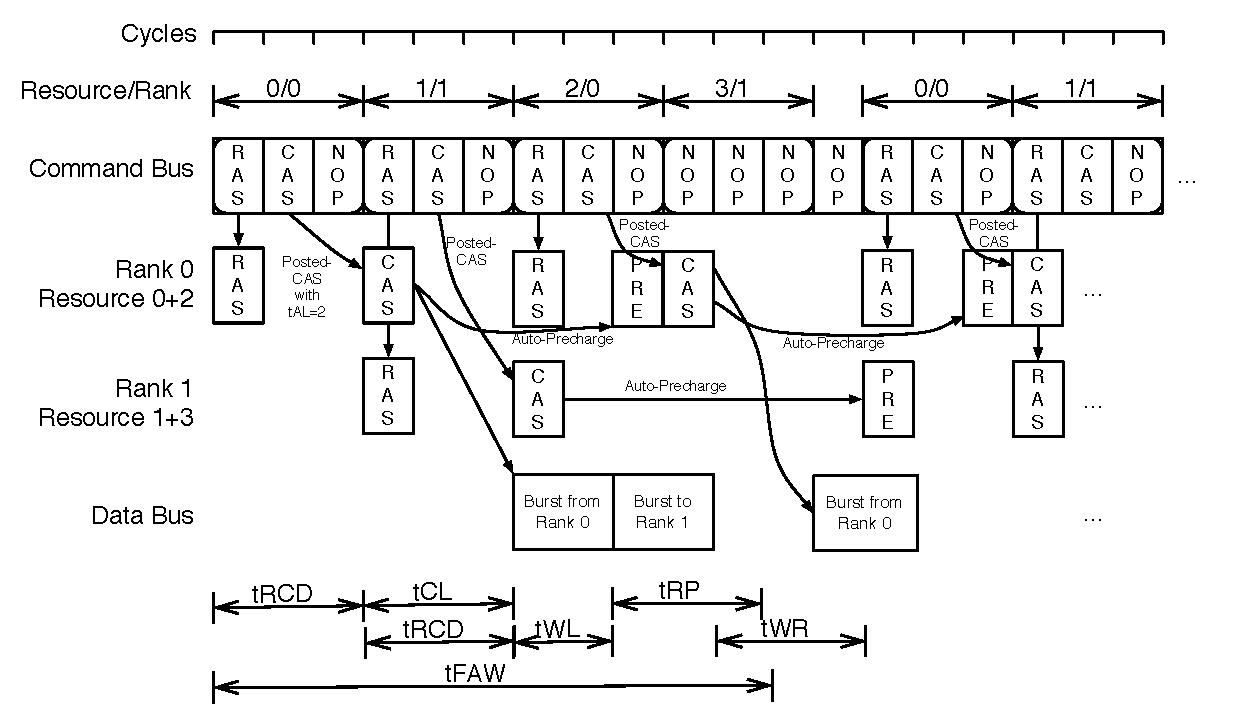
\includegraphics[width=0.92\linewidth]{figs/backend}
\end{center} 
\caption{The periodic and pipelined access scheme employed by the backend~\cite{ReinekeLiuPatelKimLee11_PRETDRAMControllerBankPrivatizationForPredictability}.}
\label{fig:backend}
\end{figure}

Each access request is translated into a RAS (Row Access), posted-CAS (Column Access) and NOP command. 
An access slot is formed of all three commands.  
The NOP command in the access slot is inserted between any two consecutive requests to avoid a collision on the data bus that occurs when a read request follows and a write request.
This collision is cause by the one cycle offset between the read and write latencies. 
The RAS command moves a row into the row buffer, and the CAS command accesses the columns within the row loaded into the row buffer. 
CAS commands can be either reads or writes, causing a burst transfer of $8 \cdot 4 = 32$ bytes that occupies the data bus for two cycles (as two transfers occur in every cycle).
We send a posted-CAS instead of a normal CAS in order to meet the row to column latency shown in table~\ref{table:ddr2-constraints}.
This latency specifies that the RAS command and the first CAS command need to be 3 cycles apart.  
However, manually issuing a CAS command to the first resource 3 cycles after its RAS command would cause a command bus conflict with the RAS command for the second resource.
Thus, we instead set the additive latency $t_{AL}$ to 2 and use the posted-CAS that offsets the CAS command to conform to the row to column latency.
This allows our memory controller to preserve our pipelined access scheme while meeting the latency requirements of the DRAM.   
We use a closed-page policy (also known as auto-precharge policy), which causes the accessed row to be immediately precharged after performing the column access (CAS), preparing it for the next row access.
If there are no requests for a resource, the backend does not send any commands to the memory module, as is the case for resource 3 in figure~\ref{fig:backend}.

Our memory design conforms to all the timing constraints listed in table~\ref{table:ddr2-constraints}.
The write-to-read timing constraint $t_{WTR}$, incurred by the sharing of I/O gating within ranks, is satisfied by alternating accesses between ranks. 
The four-bank activation window constraint is satisfied because within any window of size $t_{FAW}$ we activate at most four banks within the periodic access scheme. 
Write requests with the closed-page policy requires 13 cycles to access the row, perform a burst access, and precharge the bank to prepare for the next row access.
However, our periodic access scheme has a period of 12 cycles, as each access slot is 3 cycles, and there are four resources accessed. 
Thus, a NOP is inserted after the four access slots: to increase the distance between two access slots belonging to the same resource from 12 to 13 cycles.
As a result, the controller periodically provides access to the four resources every 13 cycles.
The backend does not issue any refresh commands to the memory module.
Instead, it relies on the frontend to refresh the DRAM cells using regular row accesses.

% \paragraph{Longer Bursts for Improved Bandwidth}
% Depending on the application, bandwidth might be more important than latency.
% Bandwidth can be improved by increasing the burst length from 4 to 8.
% Extending the proposed access scheme to a burst length of 8 is straightforward with the insertion of two additional NOP commands after each request to account for the extra two cycles of data being transfered on the data bus.  
% In this case, the access slot latency for each request is increased from three to five to include the extra two NOP commands, and data will be transferred in four out of five cycles rather than in two out of three.
% Then, of course, latency of transfers of size less than or equal to 32 bytes increases, but the latency of large transfers decreases and higher bandwidth is achieved. 

\begin{wrapfigure}{r}{0.5\textwidth}
\begin{center}
\vspace{-8mm}
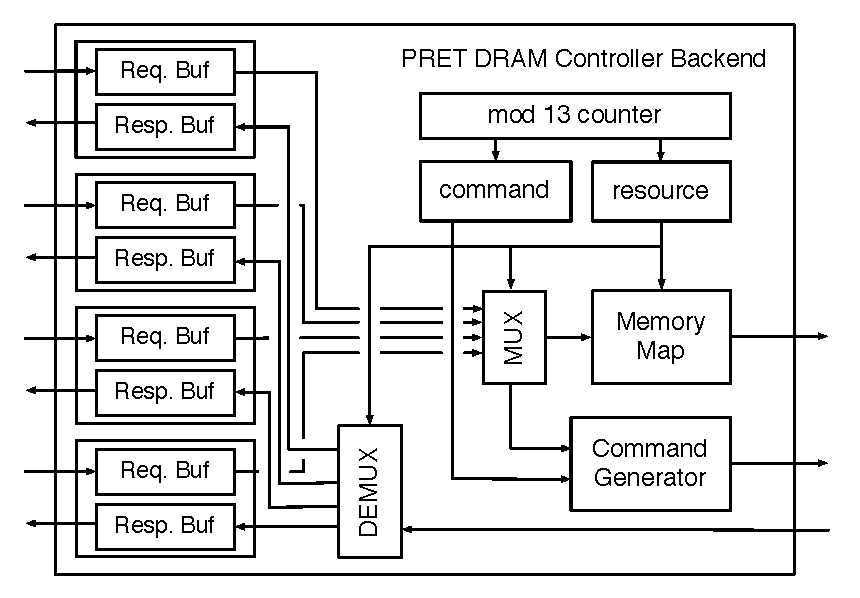
\includegraphics[width=1.1\linewidth]{figs/dram-backend-implementation}
\end{center}
\caption{Sketch of implementation of the backend~\cite{ReinekeLiuPatelKimLee11_PRETDRAMControllerBankPrivatizationForPredictability}.}
\label{fig:dram-backend-implementation}
\end{wrapfigure}

A high level block view of our backend implementation is shown in figure~\ref{fig:dram-backend-implementation}.
Each resource has a single request buffer and a respond buffer.
These buffers are used to interface with the frontend.   
A request is made of an access type (read or write), a logical address, and the data to be written for write requests. 
Requests are serviced at the granularity of bursts, i.e. 32 bytes in case of burst length 4 and 64 bytes in case of burst length 8.
A modulo-13 counter is used to implement the 13 cycle periodic access scheme in our controller.   
The ``resource'' and ``command" blocks are combinational circuits that are used to select the correct request buffer and generate the DRAM commands to be sent out. 
The ``memory map" block is where logical addresses are mapped to physical addresses that determine the rank, bank, row and column to access.
The data for read requests are latched into the response buffers to be read by the frontend.  

\paragraph{Frontend}
The frontend of our memory controller manages the interfacing to our backend, and the refreshing of the DRAM device.
The privatization of DRAM banks creates four independent resources that are accessed separately from the front end.
Thus, our memory controller is designed to be used by multicore or multithreaded architectures that contain multiple requesters which need access to the main memory.
Several recent projects, such as MERASA~\cite{Ungerer10}, PREDATOR~\cite{Akesson2007CODES}, JOP~\cite{Schoeberl2008265}, or CoMPSoC~\cite{Hansson09}, strive to develop predictable multi-core architectures that require predictable and composable memory performance.
These could potentially profit from using the proposed DRAM controller.

Specifically, we designed this memory controller to interface with the thread-interleaved pipeline discussed previously in section~\ref{section:pret_thread_pipeline}.
The thread-interleaved pipeline contains multiple hardware threads that each require access to main memory. 
We assign each hardware thread to a private memory resource, and send out memory requests to the memory controller frontend, which receives the request and places it within the request buffer.
Each thread in the thread-interleaved pipeline sends out only one outstanding memory request at a time, so the single request buffer for each resource is sufficient to interface with our thread-interleaved pipeline.
Once the request is serviced from the backend, the pipeline can read the data from the response buffer, and prepare to send another memory request.    
In section~\ref{sec:ptarm_memory} we will detail how our implemented thread-interleaved pipeline interfaces with this predictable DRAM controller, and discuss the memory access latency of this interaction.

\subparagraph{Shared Data}
The privatization of resources for predictable access means that there is no shared data in the DRAM.
This serves as an interesting design challenge, as it is impossible to assume no communication between contexts in a multicore or multithreaded environment.
In our implementation, which we will detail in section~\ref{sec:ptarm_memory}, the scratchpads can be configured to be shared between the hardware threads for communication.  
This can be done because the scratchpad and DRAM memory have distinct address regions, so no shared memory space will overlap onto the DRAM address space. 
%If conventional caches were used, which can cache
Most multi-core processors use DRAM to share data while local scratchpads or caches are private.
In this case, the sharing of data on the DRAM can be achieved by arbitrating accesses in the frontend.
The four independent resources in the backend can be combined into one, and any access to this single resource would result in four smaller accesses to all the backend resources. 
This single resource could then be shared among the different cores of a multi-core architecture using predictable arbitration mechanisms such as Round-Robin or CCSP~\cite{Akesson08} or predictable and composable ones like time-division multiple access (TDMA). 
This sharing of DRAM resources comes at a cost of increased memory access latency, which is detailed in~\cite{ReinekeLiuPatelKimLee11_PRETDRAMControllerBankPrivatizationForPredictability}. 

\subparagraph{Refreshing the DRAM}
The frontend of our memory controller also manages the refreshing of DRAM cells. 
DRAM cells need to be refreshed at least every 64 ms.
Conventionally this is done by issuing a hardware refresh command that refreshes several rows of a device at once\footnote{Internally, this still results in several consecutive row accesses.}.
Hardware refresh commands have longer refresh latencies each time a refresh is issued, but require fewer refresh commands to meet the refresh constraints posed by the DRAM.
However, when the hardware refresh command is issued, all banks in the target DRAM device are refreshed, prohibiting any other memory access to the device.
In our backend, this would extend across multiple resources, causing multiple resources to be blocked for memory accesses. 
Memory access latencies now need to account for potential refresh command latencies, which vary depending on the refresh progress.  
Instead, we use the distributed, RAS-only refresh~\cite{spec:micronddr2} to each bank separately.
Memory refreshes in this case are equivalent to row accesses to a bank; each resource can be refreshed without effecting others.
Manually accessing rows on the other give much shorter latencies each time, but incur a slight bandwidth hit because more accesses need to be performed to meet the refresh constraints.
The shorter latencies however improve the worst-case access latency, because the refresh latency is shorter.

%When a refresh is required can be statically analyzed. 
In our device, each bank consists of 8192 rows, so each row has to be refreshed every $64\textit{ms}/8192=7.8125 {\mu}s$.
At a clock rate of 200 MHz of the memory controller, this corresponds to $7.8125 {\mu}s \cdot (200 \textit{cycles}/{\mu}s) = 1562.5$ cycles.
Since each resource contains two banks, we need to perform two refreshes every $1562.5$ cycles, or one every $781.25$ cycles.
One round of access is $13$ cycles at burst length 4, and includes the access slots to each resource plus a nop command. 
So in the frontend we schedule a refresh every $\lfloor 781.25/13 \rfloor^{th} = 60^{th}$ round of the backend.
If no memory access is in the request buffer for the resource being scheduled for refresh, then the row refresh can be directly be issued. 
Conventionally, when a contention between a memory request and a refresh occurs, the refresh gets priority so the data can be retained in the DRAM cell. 
However, our refresh schedule schedules refreshes slightly more often than necessary.   
Scheduling a refresh every $60 \cdot 13$ cycles means that every row, and thus every DRAM cell, is refreshed every $60\cdot 13 \textit{ cycles}\cdot 8192\cdot 2/(200000~\textit{cycles}/\textit{ms}) \leq 63.90\textit{ms}$.
We can thus push back any of these refreshes individually by up to $0.1\textit{ms} = 20000$ cycles without violating the refreshing requirement.
So in our frontend, the memory request is serviced first (which takes 13 cycles), then the refresh is issued in the next access slot. 

In section~\ref{sec:ptarm_memory} when we detail the interaction between our thread-interleaved pipeline and the memory controller, we will show that the synchronization of the thread-interleaved pipeline to our controller backend allows us to completely hide memory refreshes in some unusable access slots lost in the synchronization.
This provides predictable access latencies for all load/store instructions to the DRAM through our DRAM controller.

%\todo{discuss DMA?}
%We will also discuss interactions with DMA units    
%For loads sent from the pipeline, the pushed back refreshes become invisible:
%as the pipeline is waiting for the data to be returned and takes some time to reach the memory stage of the next instruction, it is not able to use successive access slots of the backend, and thus it is unable to observe the refresh at all.
%With this refresh scheme, refreshes do not affect the latencies of load/store instructions, and the refreshes scheduled within DMA transfers are predictable so the latency effects of the refresh can be easily analyzed.




\section{Instruction Set Architecture Extensions}
\label{sec:programming_models}
Intro text here

\subsection{PRET Programming model Section Header}
\label{sec:pret_prog_model_sec_1}

\subsection{Pret Programming model Section Header 2}
\label{sec:pret_prog_model_sec_2}

Here is another header




\chapter{Programming Models}
\label{chapter:programming_models}
Intro text here

\subsection{PRET Programming model Section Header}
\label{sec:pret_prog_model_sec_1}

\subsection{Pret Programming model Section Header 2}
\label{sec:pret_prog_model_sec_2}

Here is another header



\chapter{Applications}
\label{chapter:app}

\section{Eliminating Side-Channel-Attacks}
\label{sec:app_side_channel_attack}

Encryption algorithms are based on strong mathematical properties to prevent attackers from deciphering the encrypted content. 
%only timing attacks
However, their implementations in software naturally introduce varying run times because of data-dependent control flow paths.
Timing attacks~\cite{Kocher96timingattacks} exploit this variability in cryptosystems and extract additional information  from executions of the cipher.
These can lead to deciphering the secret key.
Kocher describes a timing attack as a basic signal detection problem~\cite{Kocher96timingattacks}. 
The ``signal'' is the timing variation caused by the key's bits when running the cipher, while ``noise'' is the measurement inaccuracy and timing variations from other factors such as architecture unpredictability and multitasking. 
This signal to noise ratio determines the number of samples required for the attack -- the greater the ``noise,'' the more difficult the attack. 
It was generally conceived that this ``noise'' effectively masked the ``signal,'' thereby shielding encryption systems from timing attacks. 
However, practical implementations of the attack have since been presented~\cite{remoteattackspracticle,DKLMQW98,SCAsurvey} that clearly indicate the ``noise'' by itself is insufficient protection. 
In fact, the architectural unpredictability that was initially believed to prevent timing attacks was discovered to enable even more attacks.
For example, computer architects use caches, branch predictors and complex pipelines to improve the average-case performance while keeping these optimizations invisible to the programmer.
These enhancements, however, result in unpredictable and uncontrollable timing behaviors, which  were all shown to be vulnerabilities that led to side-channel attacks~\cite{2004-bernstein-cachetiming,Percival05cachemissing,Onur07predictingsecret,2009-x86timing}.

In order to not be confused with Kocher's~\cite{Kocher96timingattacks} terminology of \textit{timing attacks} on algorithmic timing differences, we classify all above attacks that exploit the timing variability of software implementation \textit{or} hardware architectures as \textit{time-exploiting attacks}. 
In our case, a \textit{timing attack} is only one possible \textit{time-exploiting attack}.
Other time-exploiting attacks include branch predictor, and cache attacks.
Examples of other side-channel attacks are power attacks~\cite{Messerges99investigationsof,Kocher99differentialpower}, fault injection attacks~\cite{biham97differential,Feng_efficientcomb}, and many others~\cite{SCAsurvey}.
%Bernstein at al.\cite{2004-bernstein-cachetiming} introduced the vulnerabilities of caches to side channel attacks; Aciicmez at al.\cite{Onur07predictingsecret} showed us how the branch predictor could be used as a side channel; 

%Attackers take advantage of different properties of the implementation such as run time, power usage, and even the behavior after manually injecting faults into the system's operation. 

In recent years, we have seen a tremendous effort to discover and counteract side-channel attacks on encryption systems~\cite{biham97differential,2009-x86timing,99designprinciples,fbscc,branchpredict,Kelsey98sidechannel,blindingrsa,cachepartition,sidechannelprocarch}.
However, it is difficult to be fully assured that all possible vulnerabilities  have been discovered.
The plethora of research on side-channel exploits~\cite{2009-x86timing,biham97differential,99designprinciples,fbscc,branchpredict,Kelsey98sidechannel,blindingrsa,cachepartition,sidechannelprocarch} indicates that we do not have the complete set of solutions as more and more vulnerabilities are still being discovered and exploited.
Just recently, Coppens et al.~\cite{2009-x86timing} discovered two previously unknown time-exploiting attacks on modern x86 processors caused by the out-of-order execution and the variable latency instructions.
This suggests that while current prevention methods are effective at \textit{defending} against their particular attacks, they do not \textit{prevent} other attacks from occurring.
This, we believe, is because they do not address the root cause of time-exploiting attacks, which is that run time variability \textit{cannot be controlled} by the programmer.

It is important to understand that the main reason for time-exploiting attacks is \textit{not} that the program runs in a varying amount of time, but that this variability \textit{cannot be controlled} by the programmer. 
The subtle difference is that if timing variability is introduced in a controlled manner, then it is still possible to control the timing information that is leaked during execution, which can be effective against time-exploiting attacks. 
However, because of the programmer's \textit{lack of control} over these timing information leaks in modern architectures, noise injection techniques are widely adopted in attempt to make the attack infeasible.
These include adding random delays~\cite{Kocher96timingattacks} or blinding signatures~\cite{Kocher96timingattacks,blindingrsa}. 
Other techniques such as branch equalization~\cite{Molnar05theprogram,SCAsurvey} use software techniques to rewrite algorithms such that they take equal time to execute during each conditional branch. 
We take a different approach, and  directly address the crux of the problem, which is the \textit{lack of control} over timing behaviors in software. 
%Computer architects have introduced caches and complex pipelines to improve the average-case performance while keeping these optimizations invisible to the programmer. 
%However, these improvements often attribute to the unpredictable and uncontrollable timing behaviors, which result in time-exploiting attacks.
We propose the use of an embedded computer architecture that is designed to allow predictable and controllable timing behaviors.

%By proposing a predictable architecture, it may seem that we are making the attacker's job easier by reducing the ``noise'' 
At first it may seem that a predictable architecture makes the attacker's task simpler, because it reduces the amount of ``noise'' emitted from the underlying architecture.
However, we contend that in order for timing behaviors to be controllable, the underlying architecture \textit{must} be predictable.
This is because it is meaningless to specify any timing semantics in software if the underlying architecture is unable to honor them.
And in order to guarantee the execution of the timing specifications, the architecture must be predictable. 
%Hiren - I removed this because it was said at the very end of the introduction
%we argue that a combination of software techniques to control execution times, and hardware techniques that make an architecture predictable are necessary to thwart time-exploiting attacks.
%\textcolor{red}{\FIXME{Sounds too casual -- rephrase}Let us also not forget that the architecture unpredictability which was once thought to shield systems from timing attacks were eventually discovered to be the main vulnerabilities in other side-channel attacks, mainly because they were uncontrollable.}
Our approach does not attempt to increase the difficulty in performing time-exploiting attacks, but to eliminate them completely. 
%As such, we argue that only by providing a timing predictable architecture, can we allow controllable timing behaviors, which removes the source of time-exploiting attacks. 

In this paper, we present the PREcision Timed (PRET) architecture~\cite{pret_cases08} in the context of embedded cryptosystems, and show that an architecture designed for predictability and controllability effectively eliminates all time-exploiting attacks.
%The PREcision Timed architecture~\cite{pret_cases08} (PRET) allows for precision timing control, and was originally proposed for real-time embedded systems.
Originally proposed by Lickly et al~\cite{pret_cases08}, PRET provides instruction-set architecture (ISA) extensions that allow programmers to control an algorithm's temporal properties at the software level.
To guarantee that the timing specifications are honored, PRET provides a predictable architecture that replaces complex pipelines and speculation units with multithread-interleaved pipelines, and replaces caches with software-managed fast access memories.  
This allows PRET to maintain predictability without sacrificing performance.
We target embedded applications such as smartcard readers~\cite{99designprinciples}, key-card gates~\cite{rfidcrypto}, set-top boxes~\cite{99designprinciples}, and thumbpods~\cite{schaumont2003tts}, which are a good fit for PRET's embedded nature.
We demonstrate the effectiveness of our approach by running both the RSA and DSA~\cite{dss} encryption algorithms on PRET, and show its immunity against time-exploiting attacks.
%The combination of ISA extensions and architectural design decision ensures that PRET can provide controllable timing semantics in software, which eliminate the vulnerability of time-exploiting attacks. 
%This makes it an appropriate match for cryptosystems.
This work shows that a disciplined defense against time-exploiting attacks requires a combination of software and hardware techniques that ensure controllability and predictability.


\section{Real Time 1D Computational Fluid Dynamics Simulator}
\label{sec:1dCFD}


\begin{figure}
  \vspace{-20pt}
  \begin{center}
    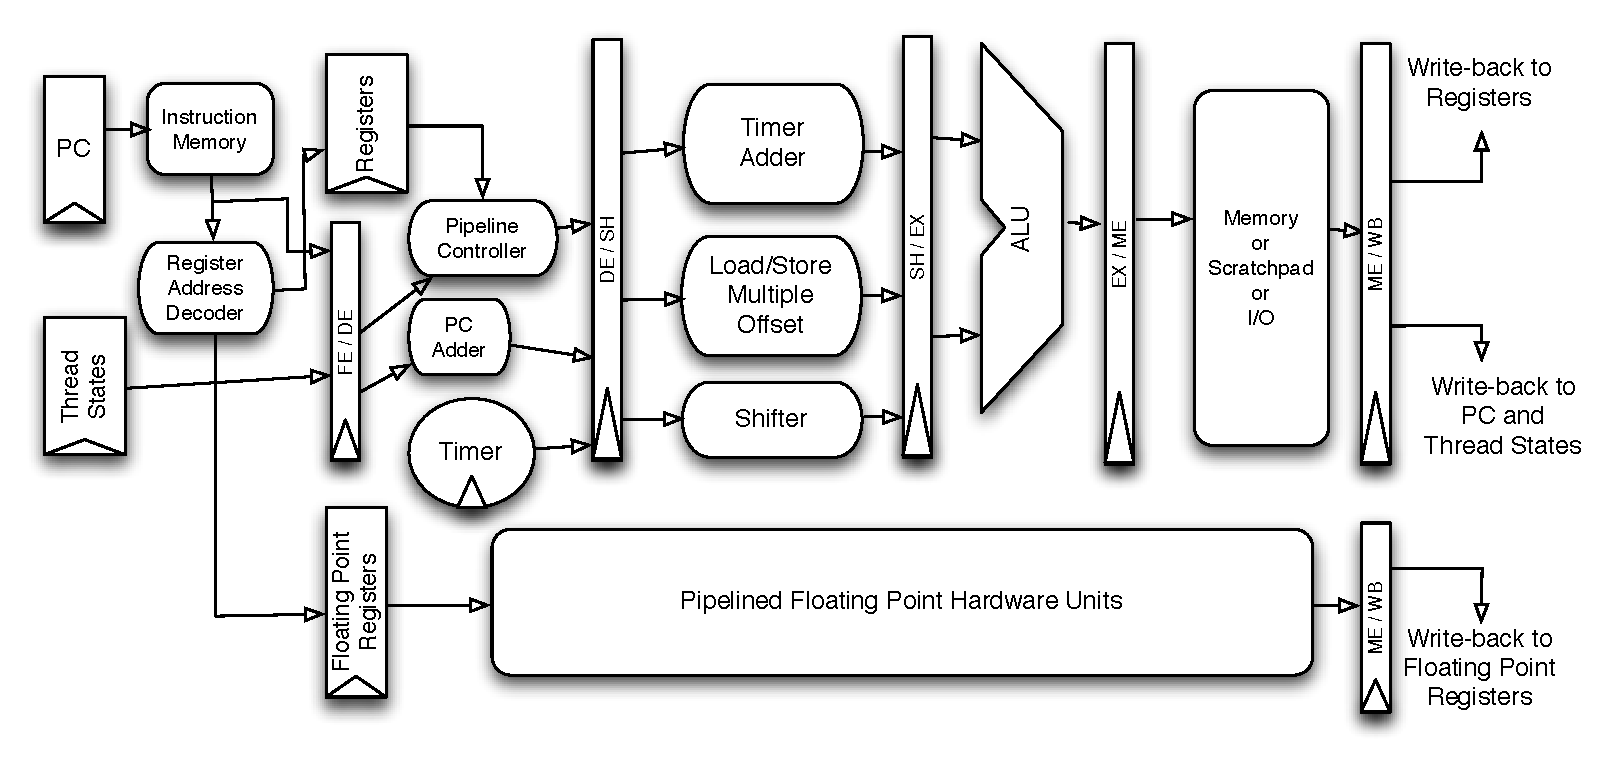
\includegraphics[scale=.6]{figs/ptarm_pipeline_six_stage}
  \end{center}
  \vspace{-20pt}
  \caption{Block Level View of the PTARM 6 stage pipeline}
  \label{fig:ptarm_pipeline_six_stage}
\end{figure}
Here is another header


\begin{figure}
\begin{center}
\vspace{-32pt}

\includegraphics[scale=.45]{figs/placeholder}
\end{center}
\vspace{-12pt}
\caption{Image Placeholder}
\label{fig:placeholder_app}
\end{figure}


\chapter{Conclusion and Future work}
\label{chapter:summary}
In order to improve the efficiency and scalability of the design of CPS and safety critical systems, we contend that changes must be made to conventional abstraction layers to introduce \emph{time} as a first class citizen.
In this thesis we focus on doing so for the ISA abstraction layer and below.  
We explore instruction extensions to the ARM ISA to bring temporal semantics to the program, independent of architecture implementation.  
We also present the precision timed ARM (PTARM), an implementation of a PRET machine, in order to provide a timing predictable and composable platform for deterministic execution times.  

To bring temporal semantics to the ISA abstraction layer, we present a few instruction extensions to the existing instruction set. 
The instructions operate on a platform clock that is synchronous with the execution of instructions. 
The instruction set extensions allow programmers to specify the timing properties of program segments, and to throw hardware exceptions when the timing specifications are not met.
In this way, our instruction extensions do not over constrain the temporal semantics of the ISA, and continue to allow architecture innovation to improve program performance. 
These extensions allow programmers to begin reasoning about temporal properties of the programs independent of the underlying execution platform, provided that the ISA is faithfully implemented.

The PTARM exploits thread-level parallelism for performance by employing a predictable thread-interleaved pipeline. 
This removes the unpredictability when handling pipeline hazards, and provides temporal isolation for all hardware threads within the pipeline.
PTARM uses scratchpads instead of caches to expose the memory hierarchy, which enables a simpler and more precise WCET analysis of memory accesses.  
With a bank privatized DRAM controller, PTARM provides predictable DRAM access latencies for each hardware thread, and preserves temporal isolation between the hardware threads that access the DRAM as a shared resource.
The timing predictability and composability provided by PTARM does not come at the cost of aggregate performance, as our benchmarks show an improved throughput for both the pipeline and DRAM memory controller when fully utilized.  
Although achieving full utilization requires that applications have sufficient concurrency, the deterministic architecture can better equip CPS platforms with the ability to handle the concurrency and the uncontrollable timing properties exhibited by physical processes.

We also demonstrate the benefits of a PRET machine in the context of a real-time engine fuel rail simulator and embedded security.
To simulate an engine fuel rail in real time, we implement a platform that uses multiple PTARM cores that communicate through local shared buffers. 
The predictable timing of PTARM allows us to statically verify that the timing constraints are met.  
The timing control provided by the extended ISA enables us to implement a software based low overhead time synchronized communication protocol between the hardware threads, saving the resources required to implement a full hardware interconnection system.
These features of PTARM enable us to implement a scalable solution that can simulate, in real time, a 237 node common fuel rail systems in a single Xinlinx Virtex 6 FPGA. 
In the context of embedded security, the underlying architecture implementing encryption algorithms is susceptible to timing side-channel attacks.
Attackers can exploit the uncontrollable execution time variances caused by the architecture or algorithm to derive the key. 
We implement the RSA and DSA encryption algorithms on a PRET architecture, and show that a predictable architecture with controllable timing properties in the ISA not only defends against all timing related side-channel attacks, but eliminates the root cause of them. 

We continue to investigate the several challenges and questions mentioned in this thesis.
First, we continue to explore the formalization of the timing extensions to the ISA. 
The introduction of temporal semantics in the ISA should be platform independent; our implementation in PTARM merely opens up opportunities for further experimentation and research. 
Nailing down the formal semantics of each instruction extension is key to a consistent meaning of ``time'' that is independent of the underlying hardware implementation. 
Second, we continue to experiment with how a predictable pipeline and memory controller handles external interrupts and I/O devices.     
With the plethora of complex interfaces and protocols for modern high speed I/O interactions, typical I/O controllers are implemented in hardware.
However, we envision a predictable architecture with precise timing control can enable software implementations of protocols typically implemented in hardware due to the lack of precise control over timing in software.
A software implementation can enable flexibility for different protocols and reduce design effort, leading to faster time-to-market and more feature rich designs.        
Third, we continue to explore the interfacing with a timing predictable bus or interconnect, which can be used in timing predictable multicore systems.
In our real-time engine fuel rail simulator, we show a multicore implementation with PRET architectures that uses local shared memories for communication and  a timing based synchronization communication protocol implemented in software.  
However, as communication schemes and applications get more complex, the interconnect or bus will play a more integral role in the connection and communication of multiple PRET cores.
Thus, our future work also includes predictable communication protocols across interconnects and shared buses that leverage the predictable timing of the PRET architecture.     

It is important to understand that we are not proclaiming that all dynamic behavior in systems are harmful.
However, the dynamic behavior must be controllable and predictable. 
For example, dynamically scheduling hardware threads in the architecture causes uncontrollable timing interference because the triggering of thread switches is hidden from, and cannot be explicitly controlled by, the programmer.
We argue that only by achieving predictability in the architecture and platforms can we begin to reason about more dynamic behavior in software.
With a predictable architecture and the introduction of temporal semantics in the ISA, we hope to provide a timing deterministic foundation in the lower levels of abstraction.
In doing so, we enable larger and more complex designs of cyber-physical systems to gain more precise and efficient control over the timing properties of the system.  



\bibliographystyle{abbrv}
\bibliography{thesis}  

% That's all folks!
\end{document}
